% !TeX root = thesis.tex
%
% Every figure in this appendix is produced by the plotting cell at the end of
% data_augmentation.ipynb. Re-run that cell to regenerate them.

\chapter{Fault Injection Verification Plots} \label{app:fault_plots}

This appendix complements Section~\ref{sec:fault_scenarios}. The main text illustrates each of the four
fault types at medium severity, on Session 16 only, together with one of the two combined scenarios. This
appendix reports every remaining combination, so that the injected signal can be inspected for all four
fault types, all three severity levels, both combined scenarios and both false positive scenarios, in each
of the two sessions used for fault injection.

Every figure follows the same convention. The grey dashed line is the original, fault-free signal of the
main sensor for that scenario, and the red line is the same signal after injection. The horizontal dotted
lines mark the manufacturer's warning and trip thresholds for that sensor, and the shaded region marks the
active fault window, that is, the interval labelled as an injected anomaly. The decay that follows the end
of the window is visible in the red line but deliberately falls outside the shaded region, since it is a
physical fade back towards the baseline rather than part of the fault itself.

Only the main sensor of each scenario is shown. The deviation propagated to the correlated sensors, as
described in Section~\ref{sec:fault_single}, is present in the generated files but is not reproduced here,
since it follows the shape of the main sensor scaled by each sensor's own correlation coefficient.

\section{Single Fault Scenarios — Session 16} \label{app:fault_s16}

The medium severity of each fault type on this session is already shown in the main text
(Section~\ref{sec:fault_single}). The remaining severities are shown below.

\begin{figure}[htbp]
    \centering
    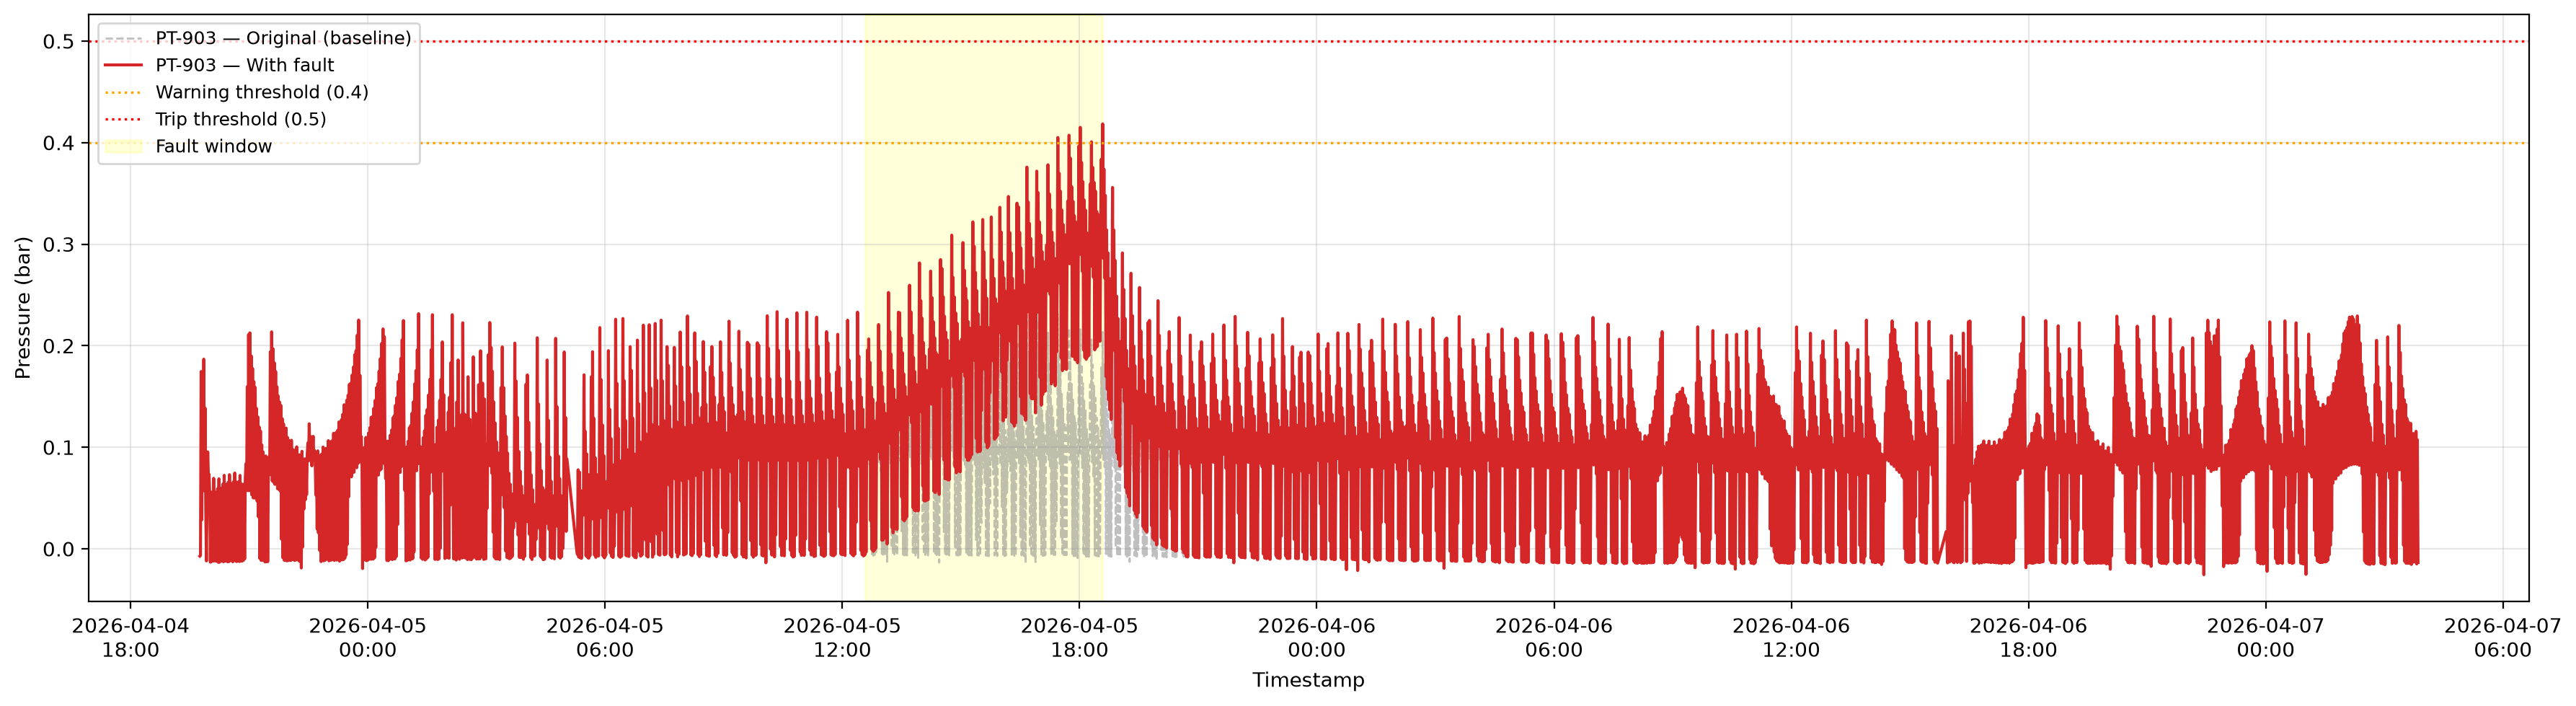
\includegraphics[width=0.95\textwidth]{imgs/fault_f1_small_s16.png}
    \caption{F1 (clogged exhaust filters), small severity, Session 16: PT-903 with and without the injected fault. The fault lasts 6 hours, starting 30\% of the way through the session.}
    \label{fig:ap2_f1_small_s16}
\end{figure}

\begin{figure}[htbp]
    \centering
    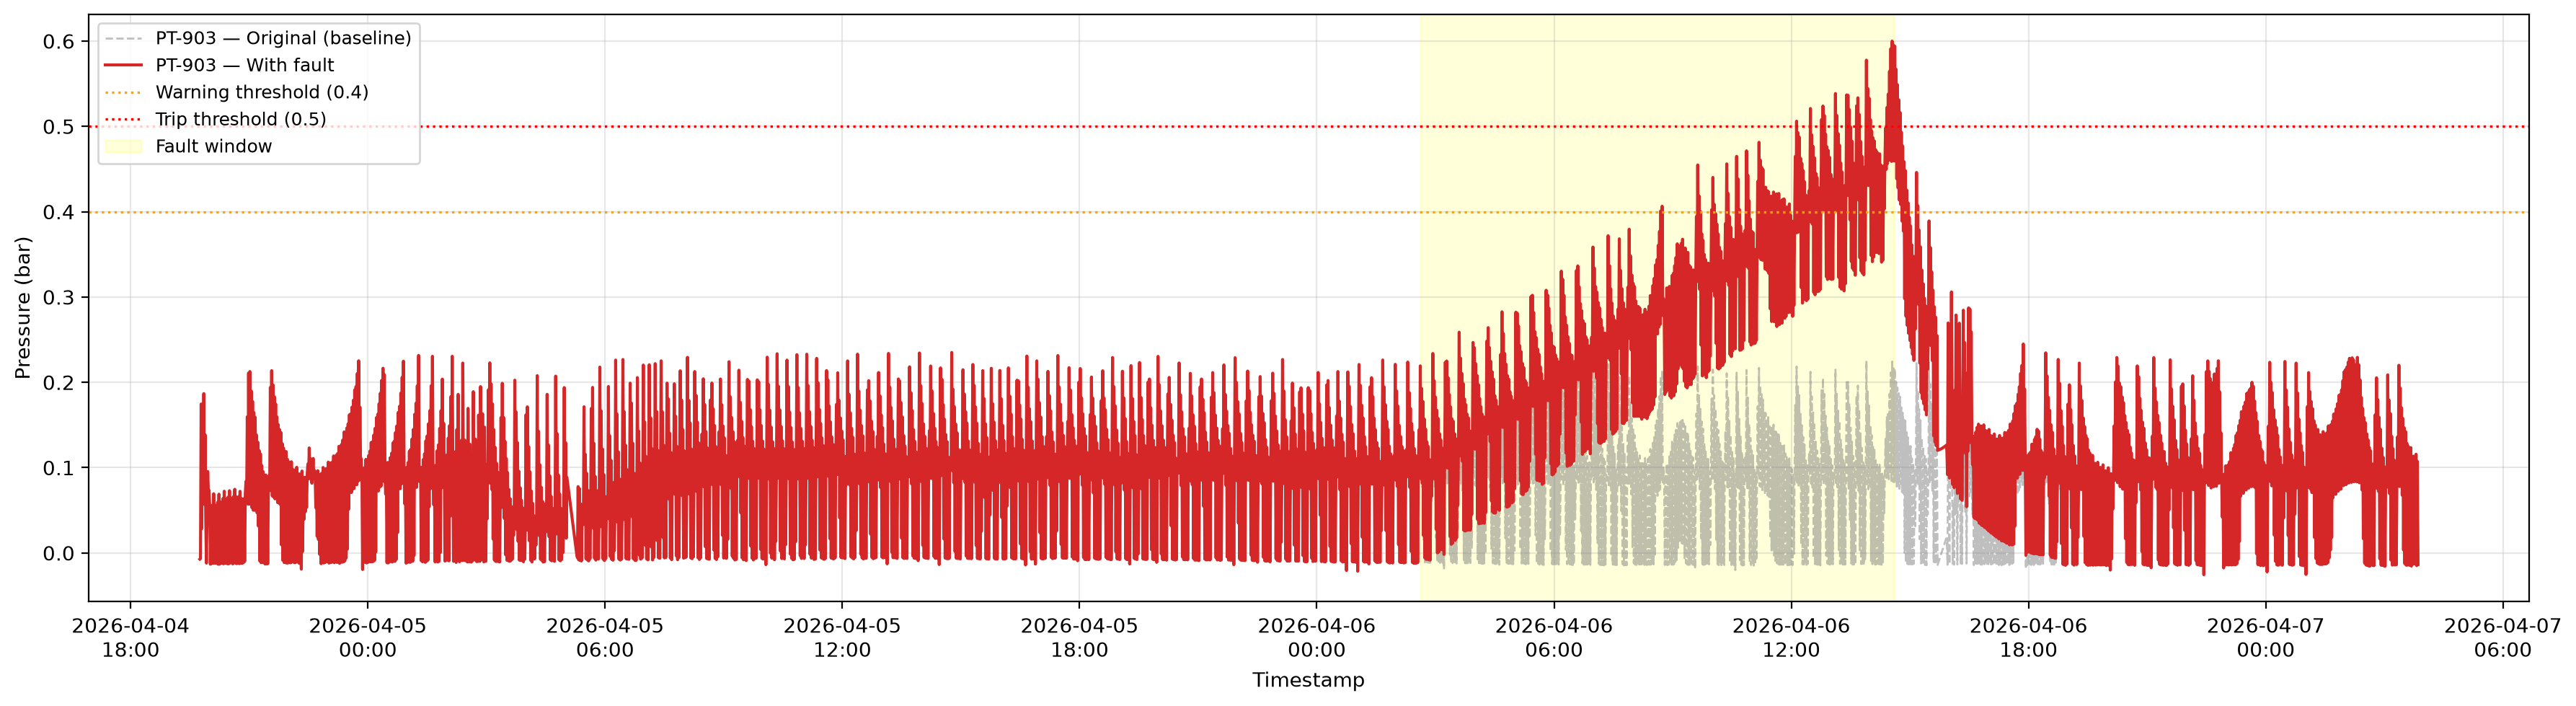
\includegraphics[width=0.95\textwidth]{imgs/fault_f1_severe_s16.png}
    \caption{F1 (clogged exhaust filters), severe severity, Session 16: PT-903 with and without the injected fault. The fault lasts 12 hours, starting 55\% of the way through the session.}
    \label{fig:ap2_f1_severe_s16}
\end{figure}

\begin{figure}[htbp]
    \centering
    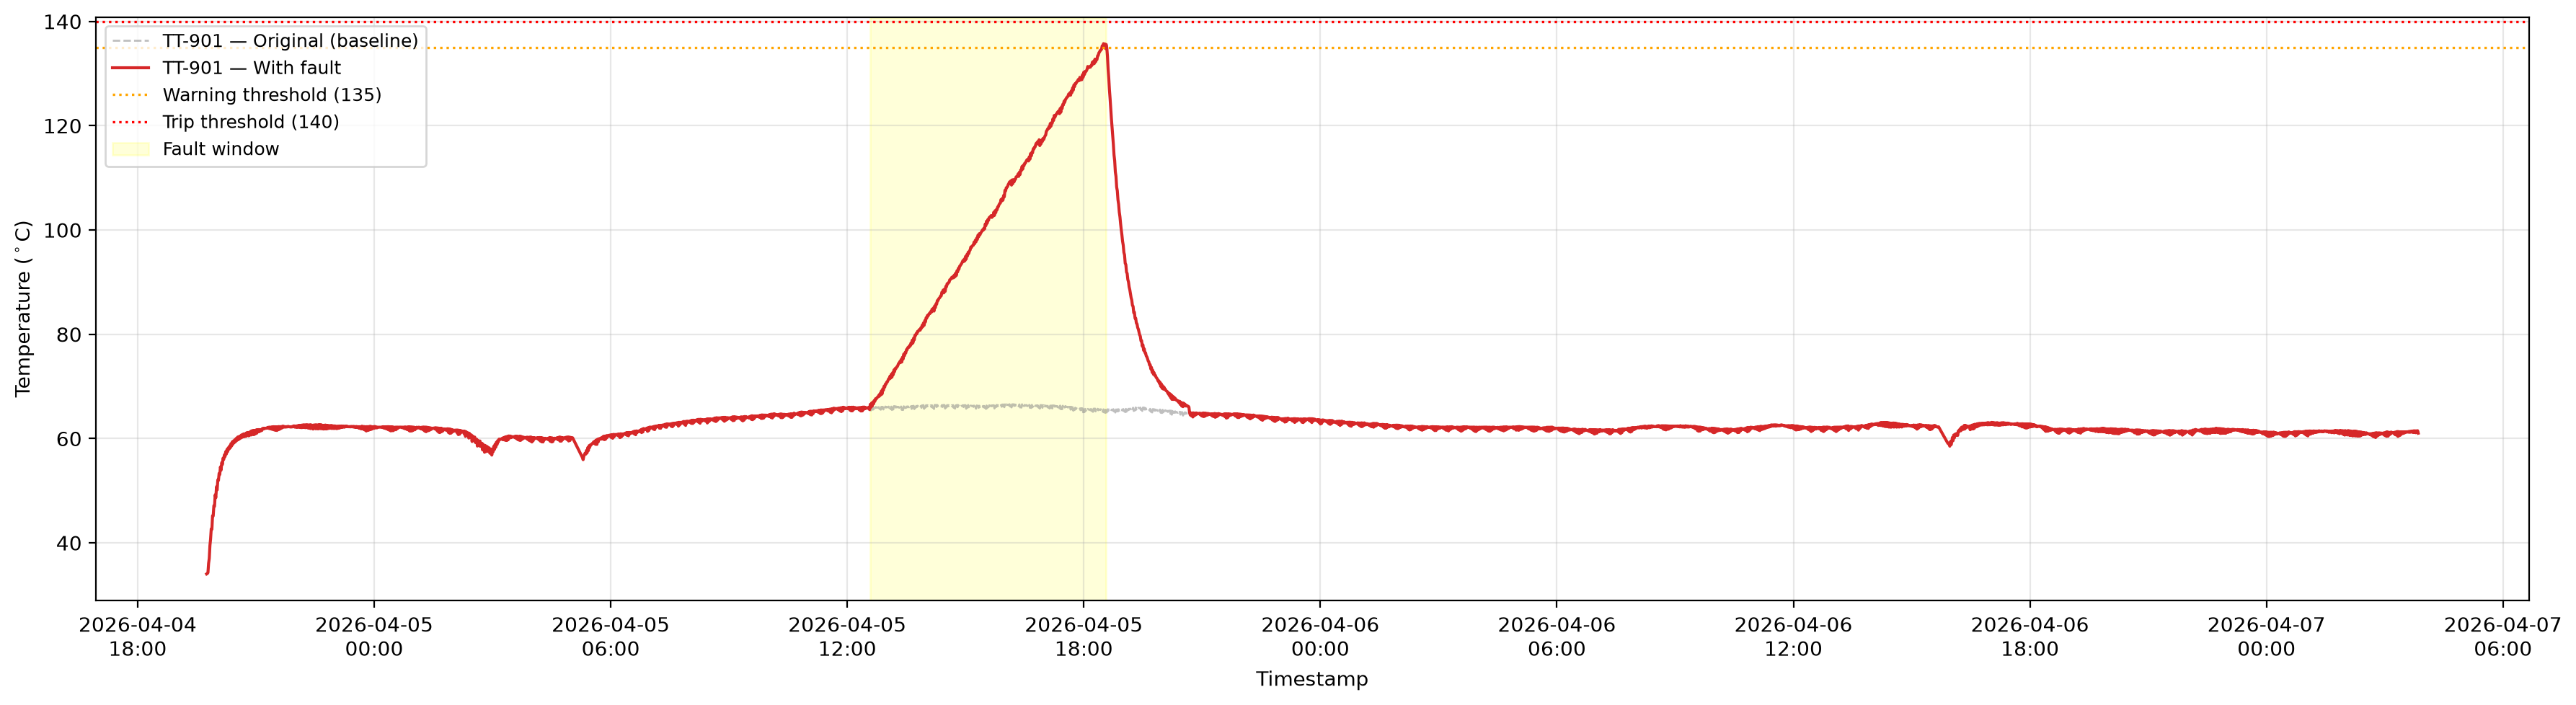
\includegraphics[width=0.95\textwidth]{imgs/fault_f2_small_s16.png}
    \caption{F2 (insufficient cooling), small severity, Session 16: TT-901 with and without the injected fault. The fault lasts 6 hours, starting 30\% of the way through the session.}
    \label{fig:ap2_f2_small_s16}
\end{figure}

\begin{figure}[htbp]
    \centering
    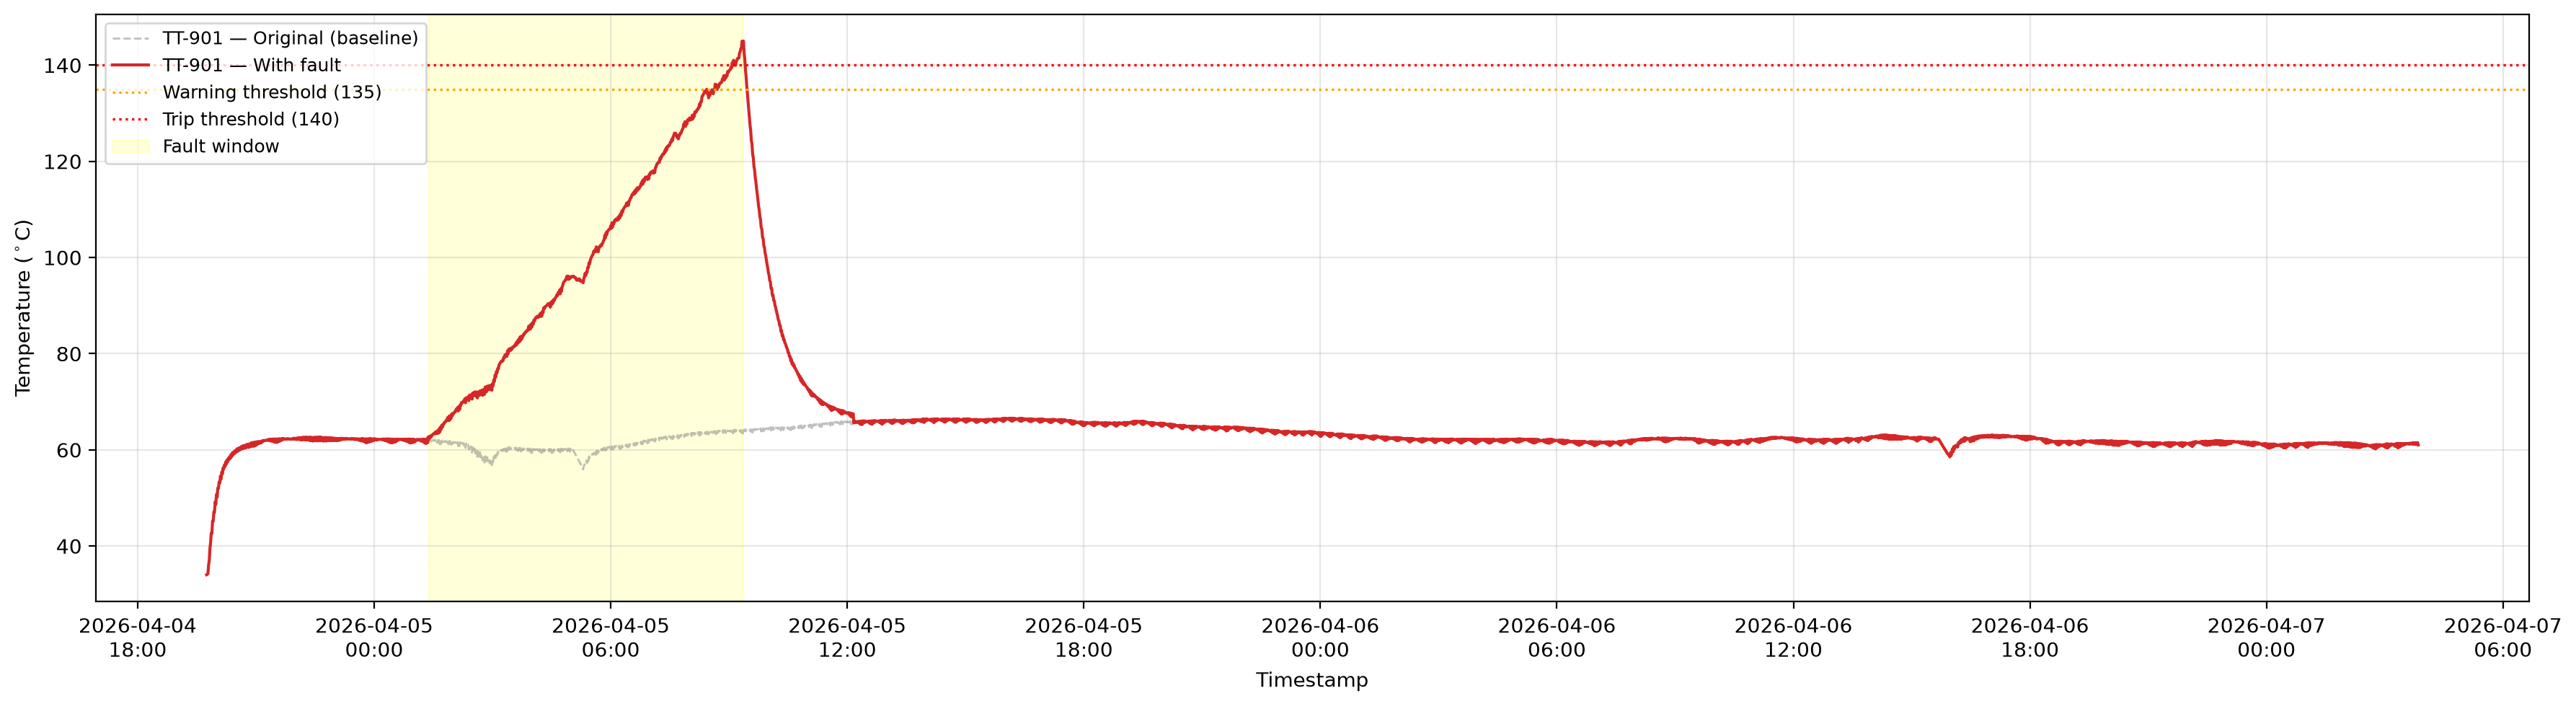
\includegraphics[width=0.95\textwidth]{imgs/fault_f2_severe_s16.png}
    \caption{F2 (insufficient cooling), severe severity, Session 16: TT-901 with and without the injected fault. The fault lasts 8 hours, starting 10\% of the way through the session.}
    \label{fig:ap2_f2_severe_s16}
\end{figure}

\begin{figure}[htbp]
    \centering
    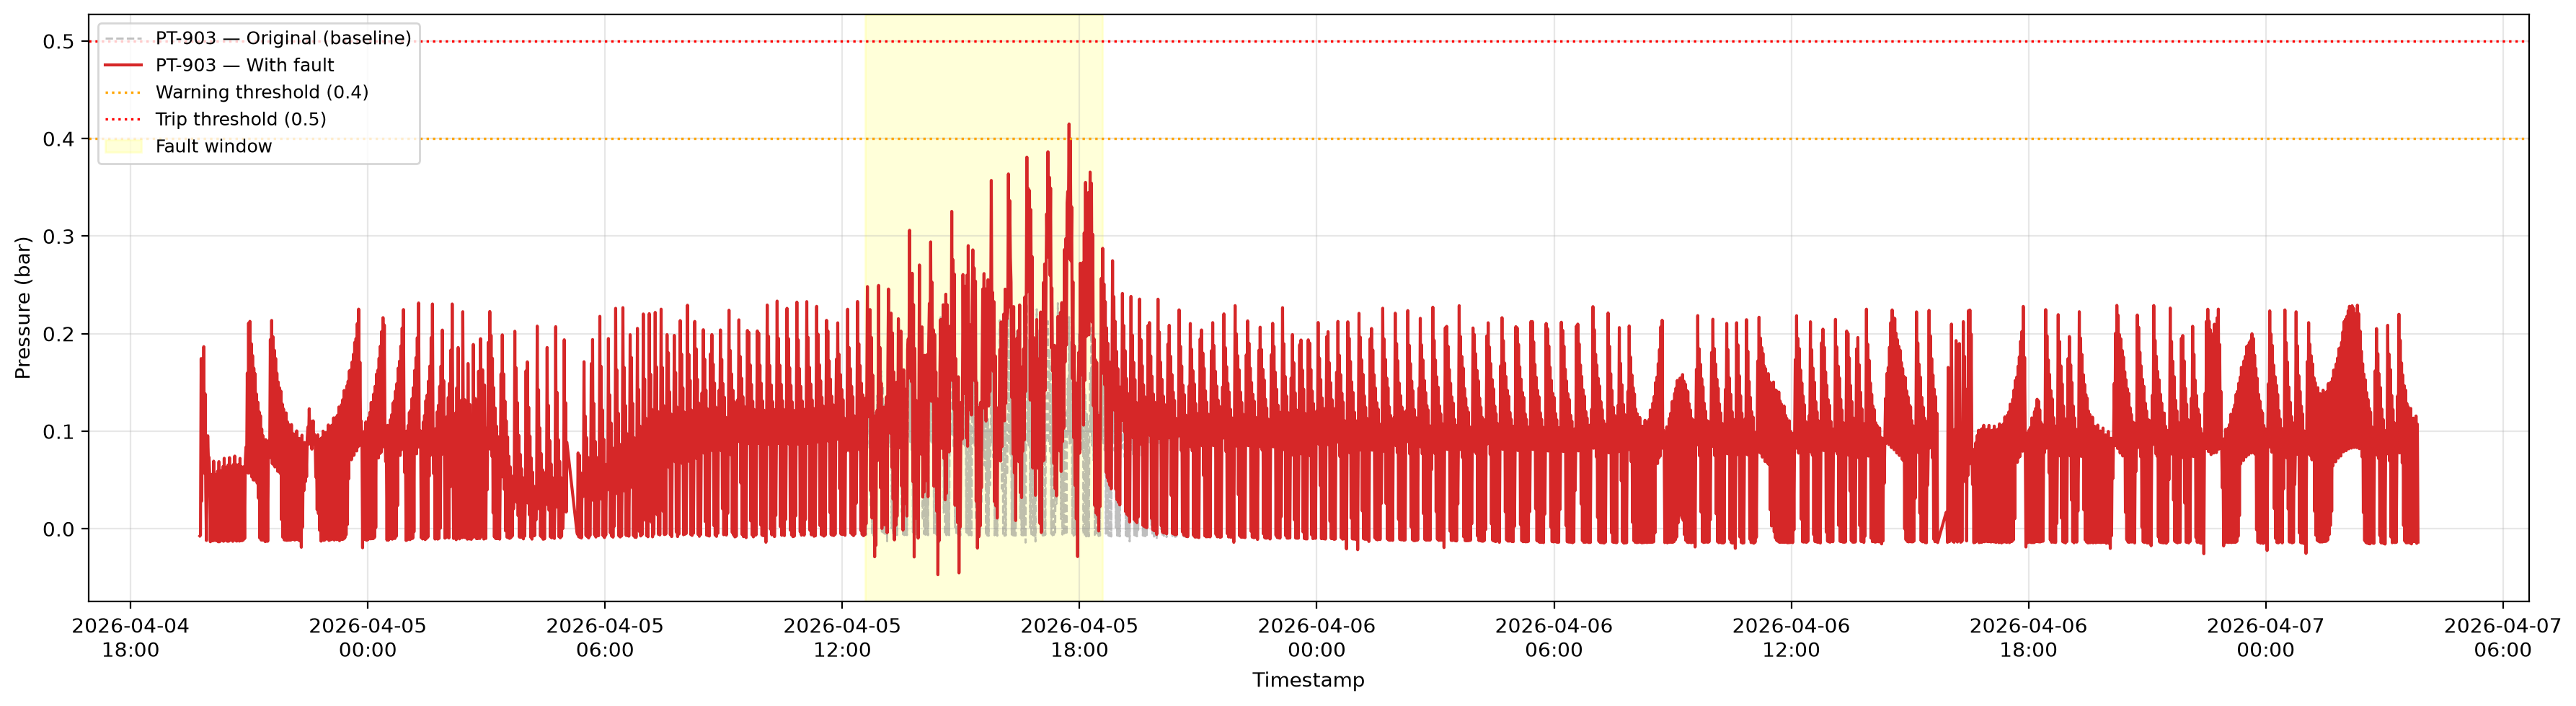
\includegraphics[width=0.95\textwidth]{imgs/fault_f3_small_s16.png}
    \caption{F3 (float valve fault), small severity, Session 16: PT-903 with and without the injected fault. The fault lasts 6 hours, starting 30\% of the way through the session.}
    \label{fig:ap2_f3_small_s16}
\end{figure}

\begin{figure}[htbp]
    \centering
    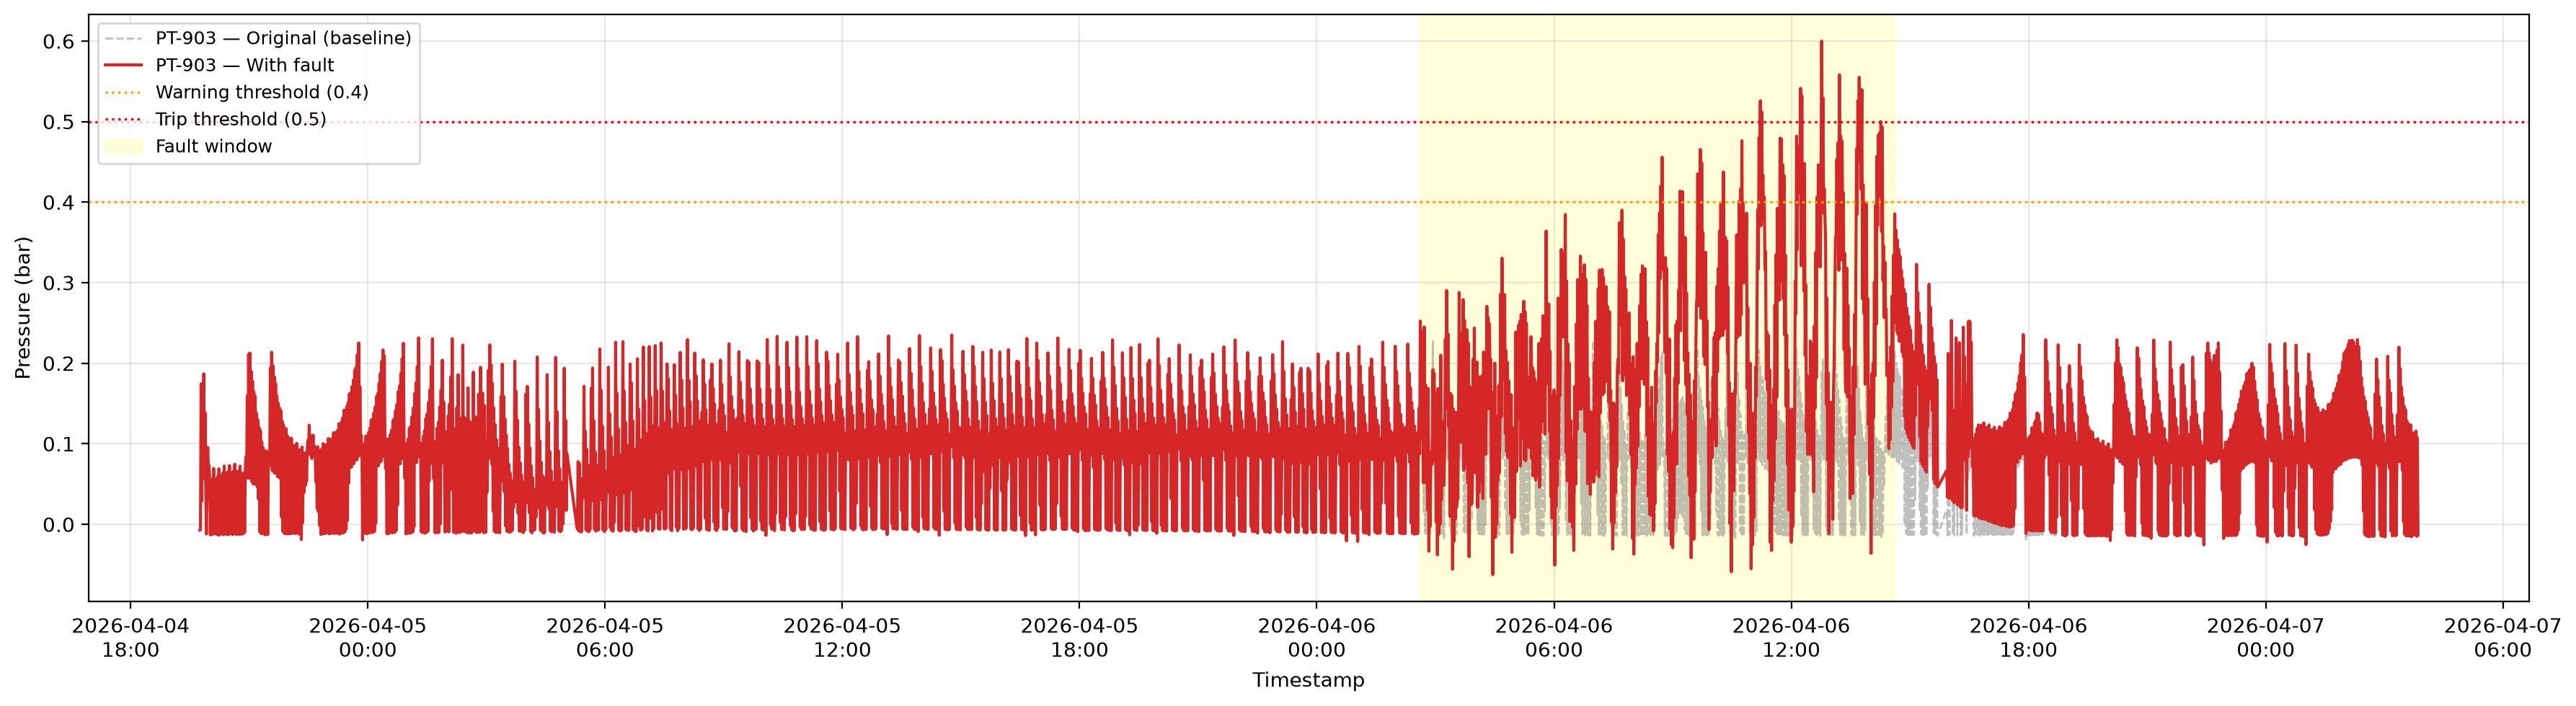
\includegraphics[width=0.95\textwidth]{imgs/fault_f3_severe_s16.png}
    \caption{F3 (float valve fault), severe severity, Session 16: PT-903 with and without the injected fault. The fault lasts 12 hours, starting 55\% of the way through the session.}
    \label{fig:ap2_f3_severe_s16}
\end{figure}

\begin{figure}[htbp]
    \centering
    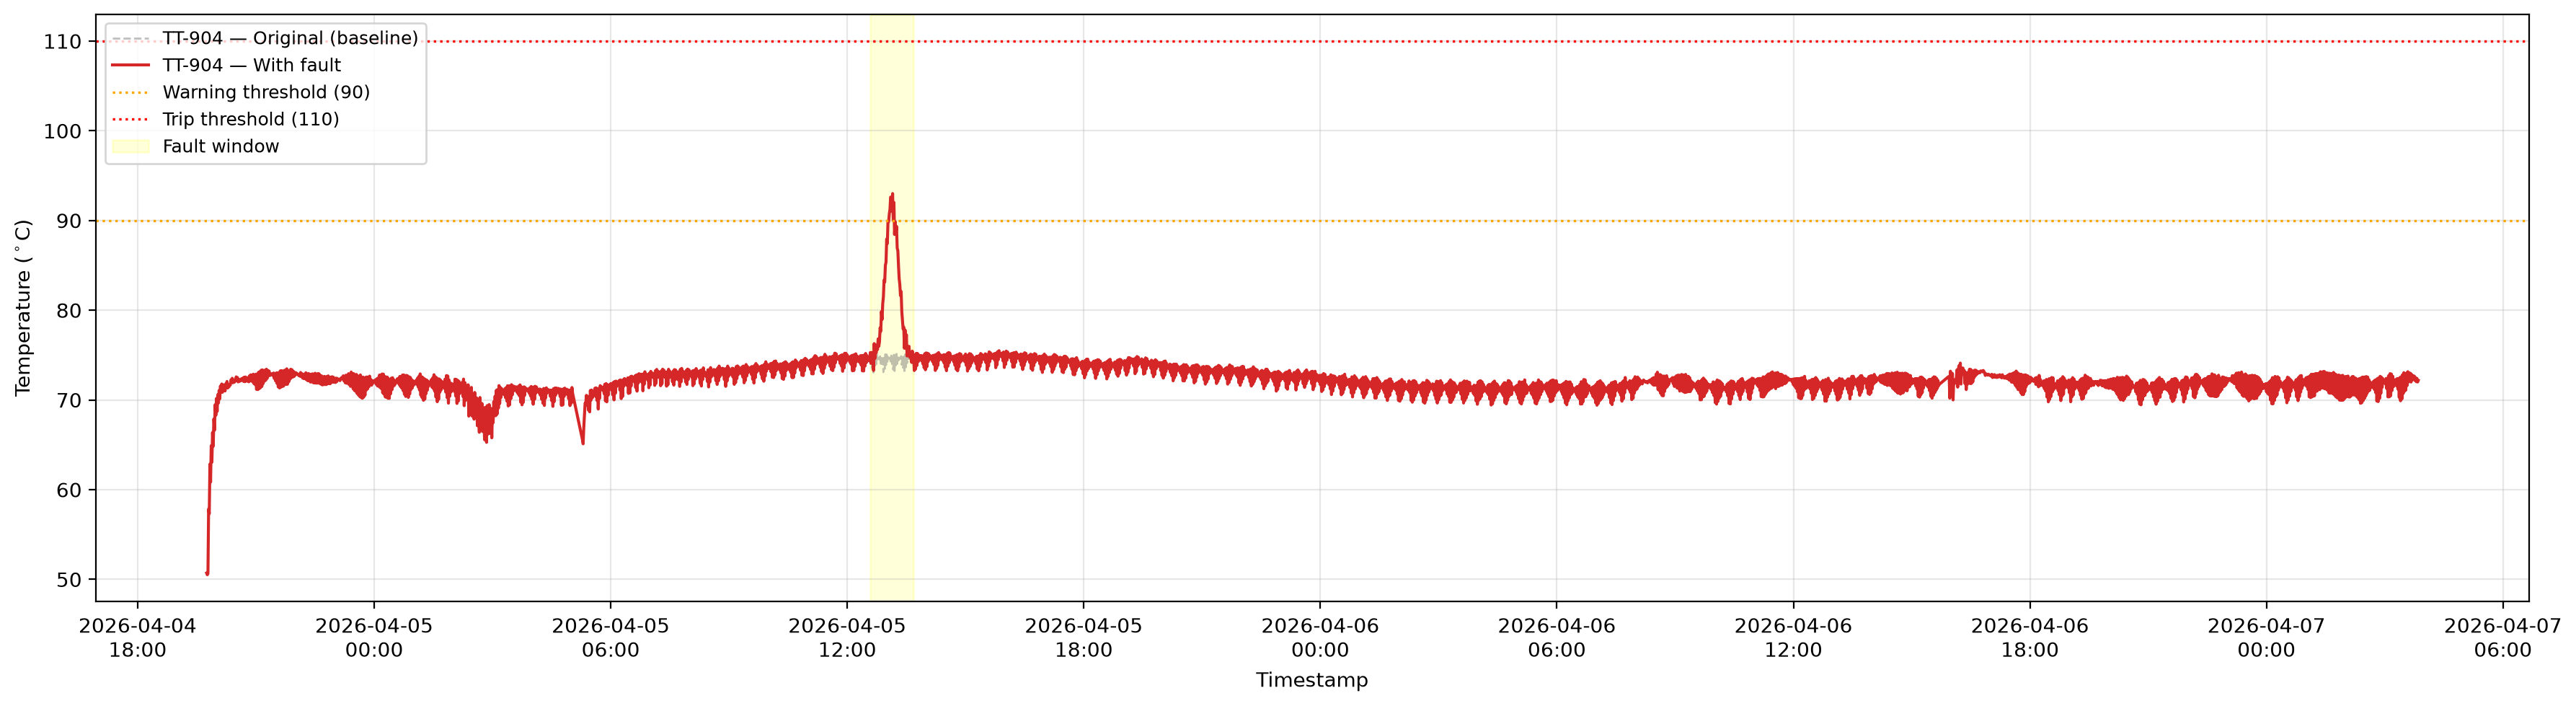
\includegraphics[width=0.95\textwidth]{imgs/fault_f4_small_s16.png}
    \caption{F4 (defective bearing), small severity, Session 16: TT-904 with and without the injected fault. The fault lasts 67 minutes, starting 30\% of the way through the session.}
    \label{fig:ap2_f4_small_s16}
\end{figure}

\begin{figure}[htbp]
    \centering
    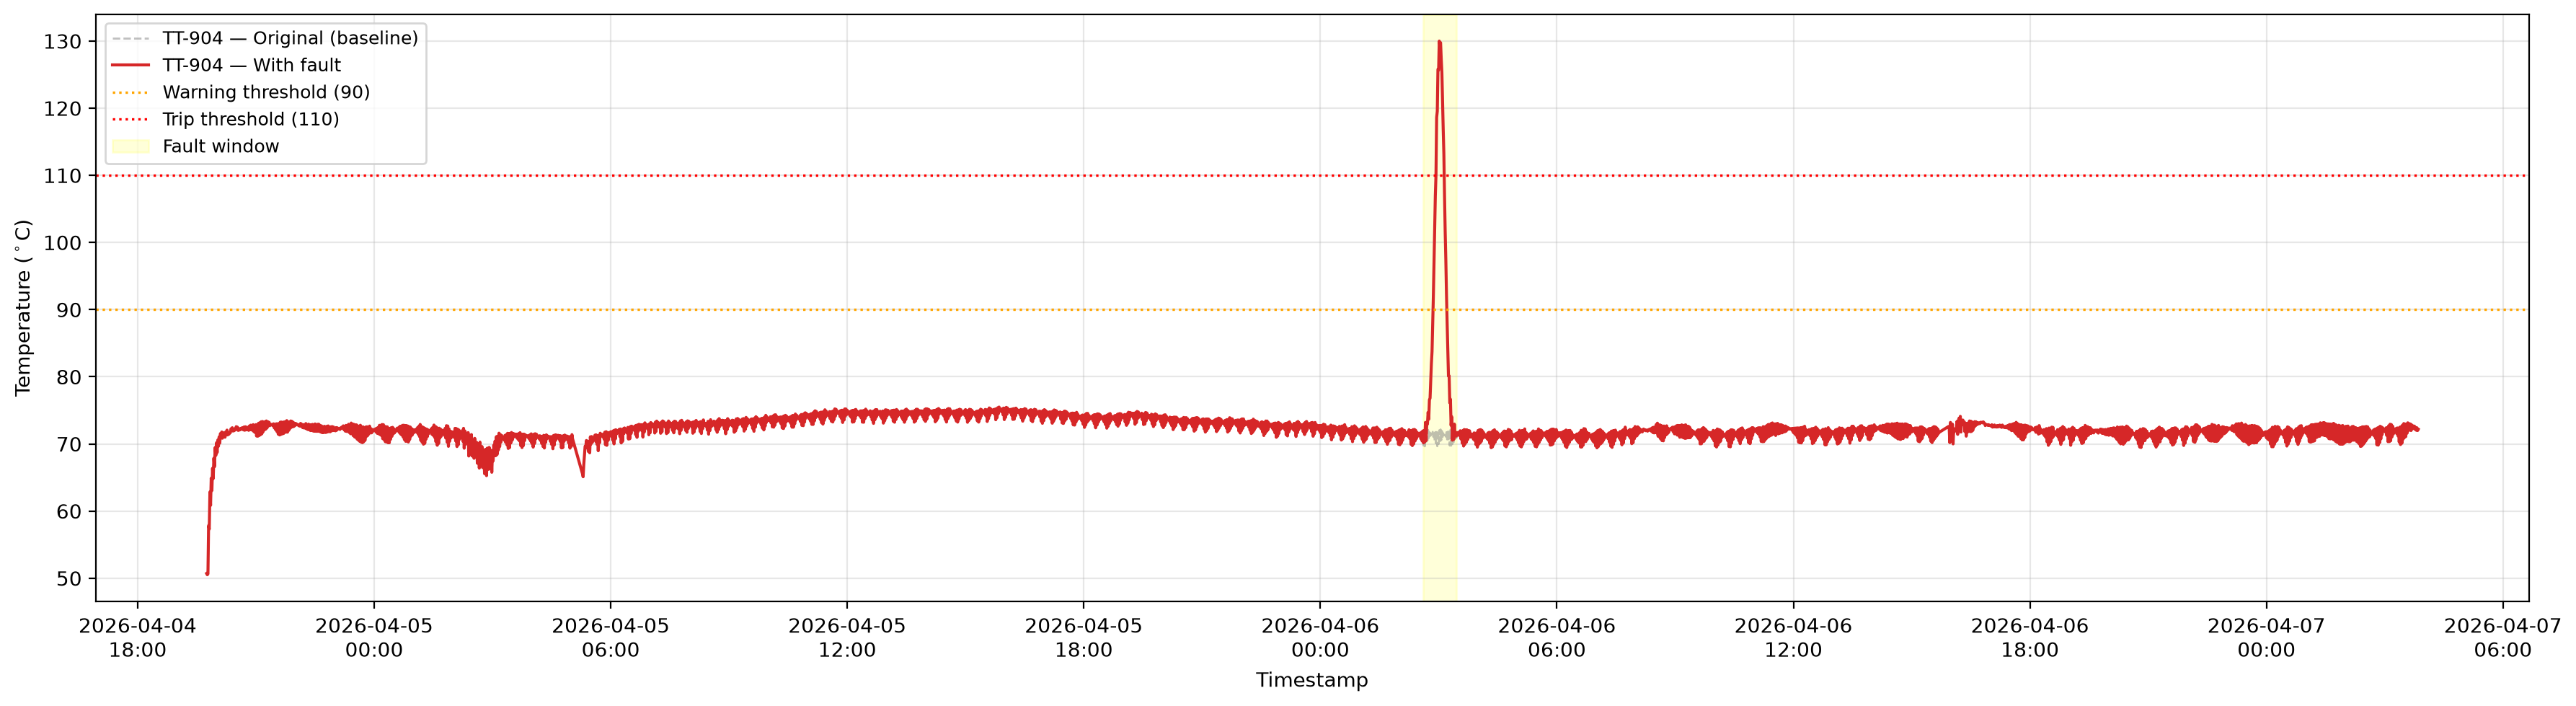
\includegraphics[width=0.95\textwidth]{imgs/fault_f4_severe_s16.png}
    \caption{F4 (defective bearing), severe severity, Session 16: TT-904 with and without the injected fault. The fault lasts 51 minutes, starting 55\% of the way through the session.}
    \label{fig:ap2_f4_severe_s16}
\end{figure}


\section{Single Fault Scenarios — Session 17} \label{app:fault_s17}

The same twelve scenarios generated from Session 17. Because the fault window is defined as a fraction of
the session length, and Session 17 is longer than Session 16 (4{,}415 against 3{,}367 observations), the
windows start at different absolute times in the two sessions even though the fault definitions are
identical.

\begin{figure}[htbp]
    \centering
    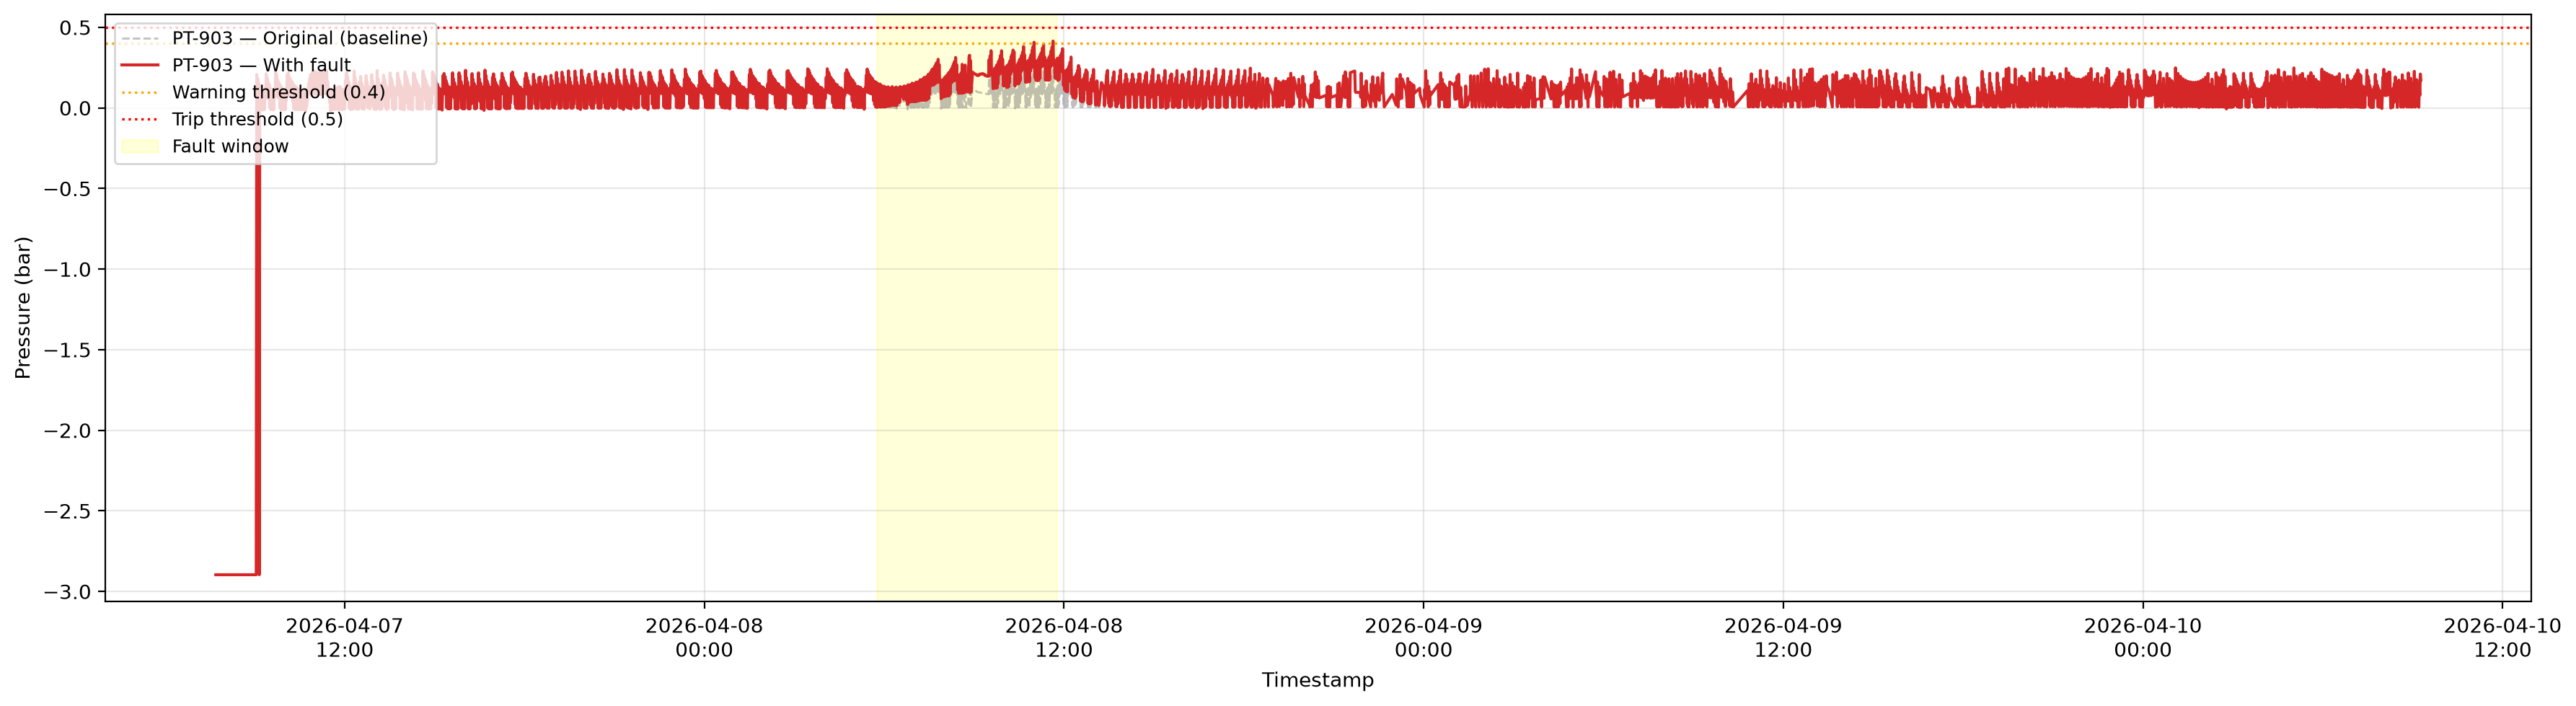
\includegraphics[width=0.95\textwidth]{imgs/fault_f1_small_s17.png}
    \caption{F1 (clogged exhaust filters), small severity, Session 17: PT-903 with and without the injected fault. The fault lasts 6 hours, starting 30\% of the way through the session.}
    \label{fig:ap2_f1_small_s17}
\end{figure}

\begin{figure}[htbp]
    \centering
    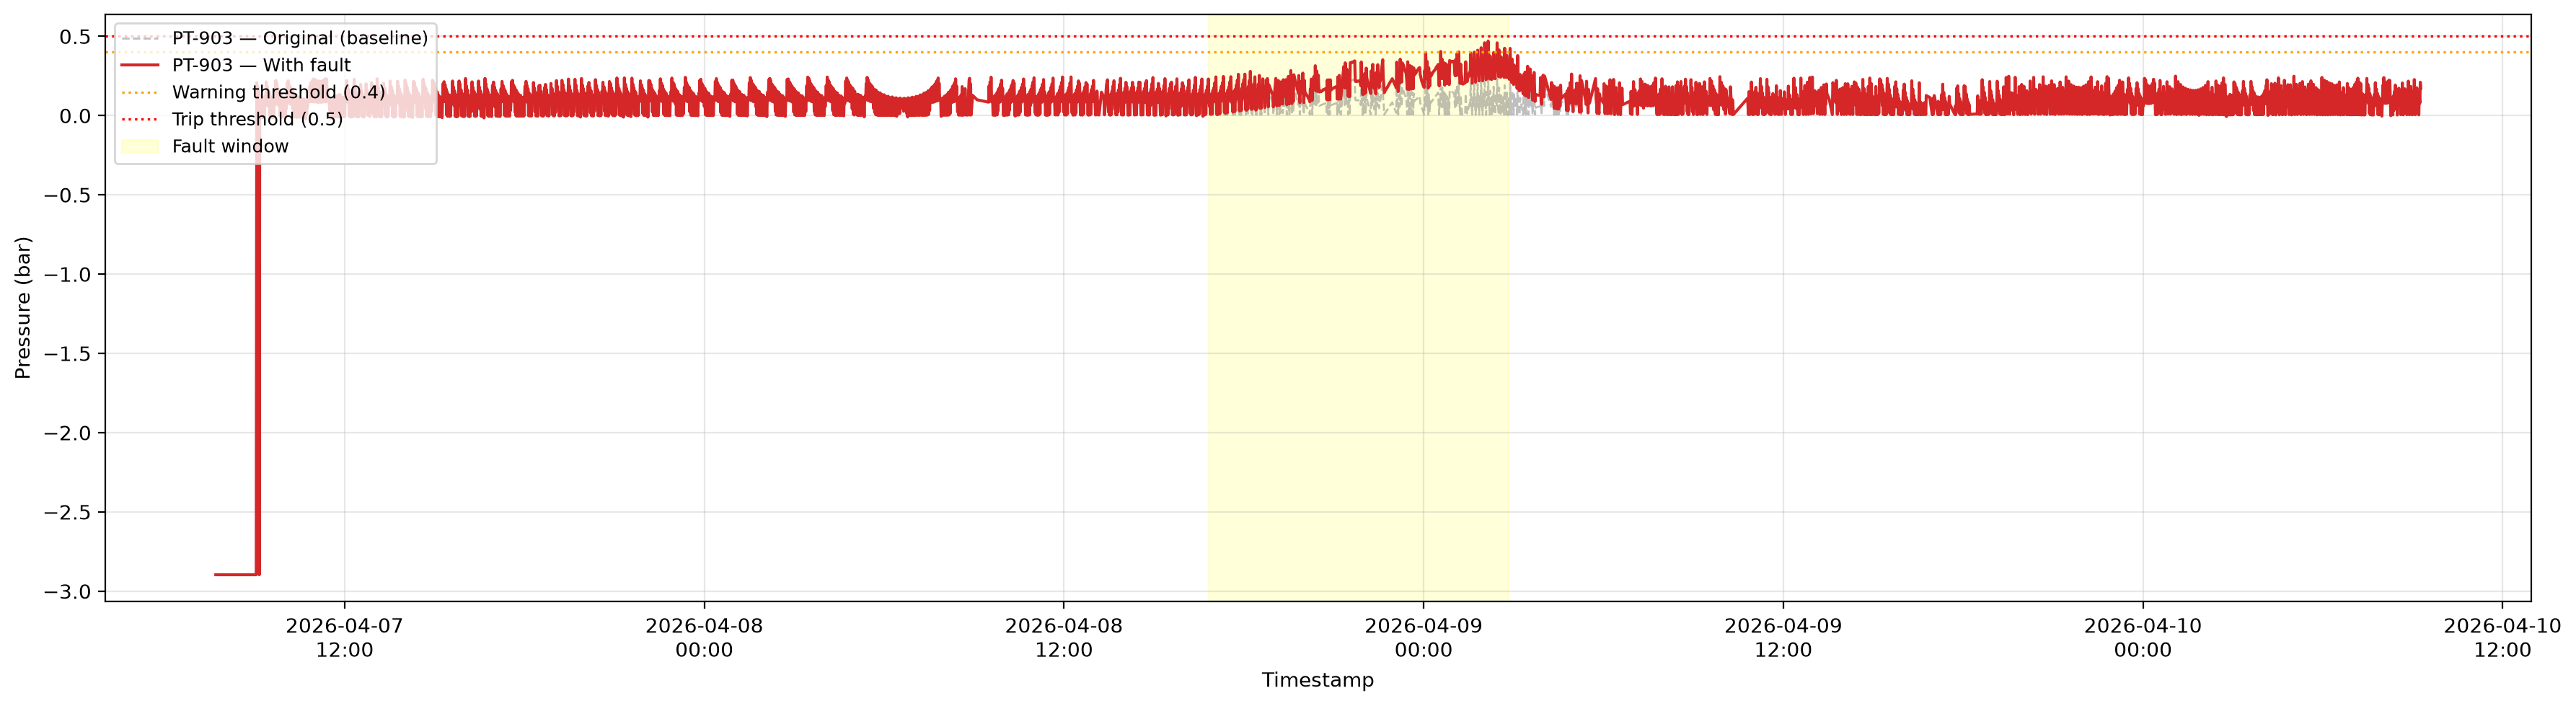
\includegraphics[width=0.95\textwidth]{imgs/fault_f1_medium_s17.png}
    \caption{F1 (clogged exhaust filters), medium severity, Session 17: PT-903 with and without the injected fault. The fault lasts 10 hours, starting 45\% of the way through the session.}
    \label{fig:ap2_f1_medium_s17}
\end{figure}

\begin{figure}[htbp]
    \centering
    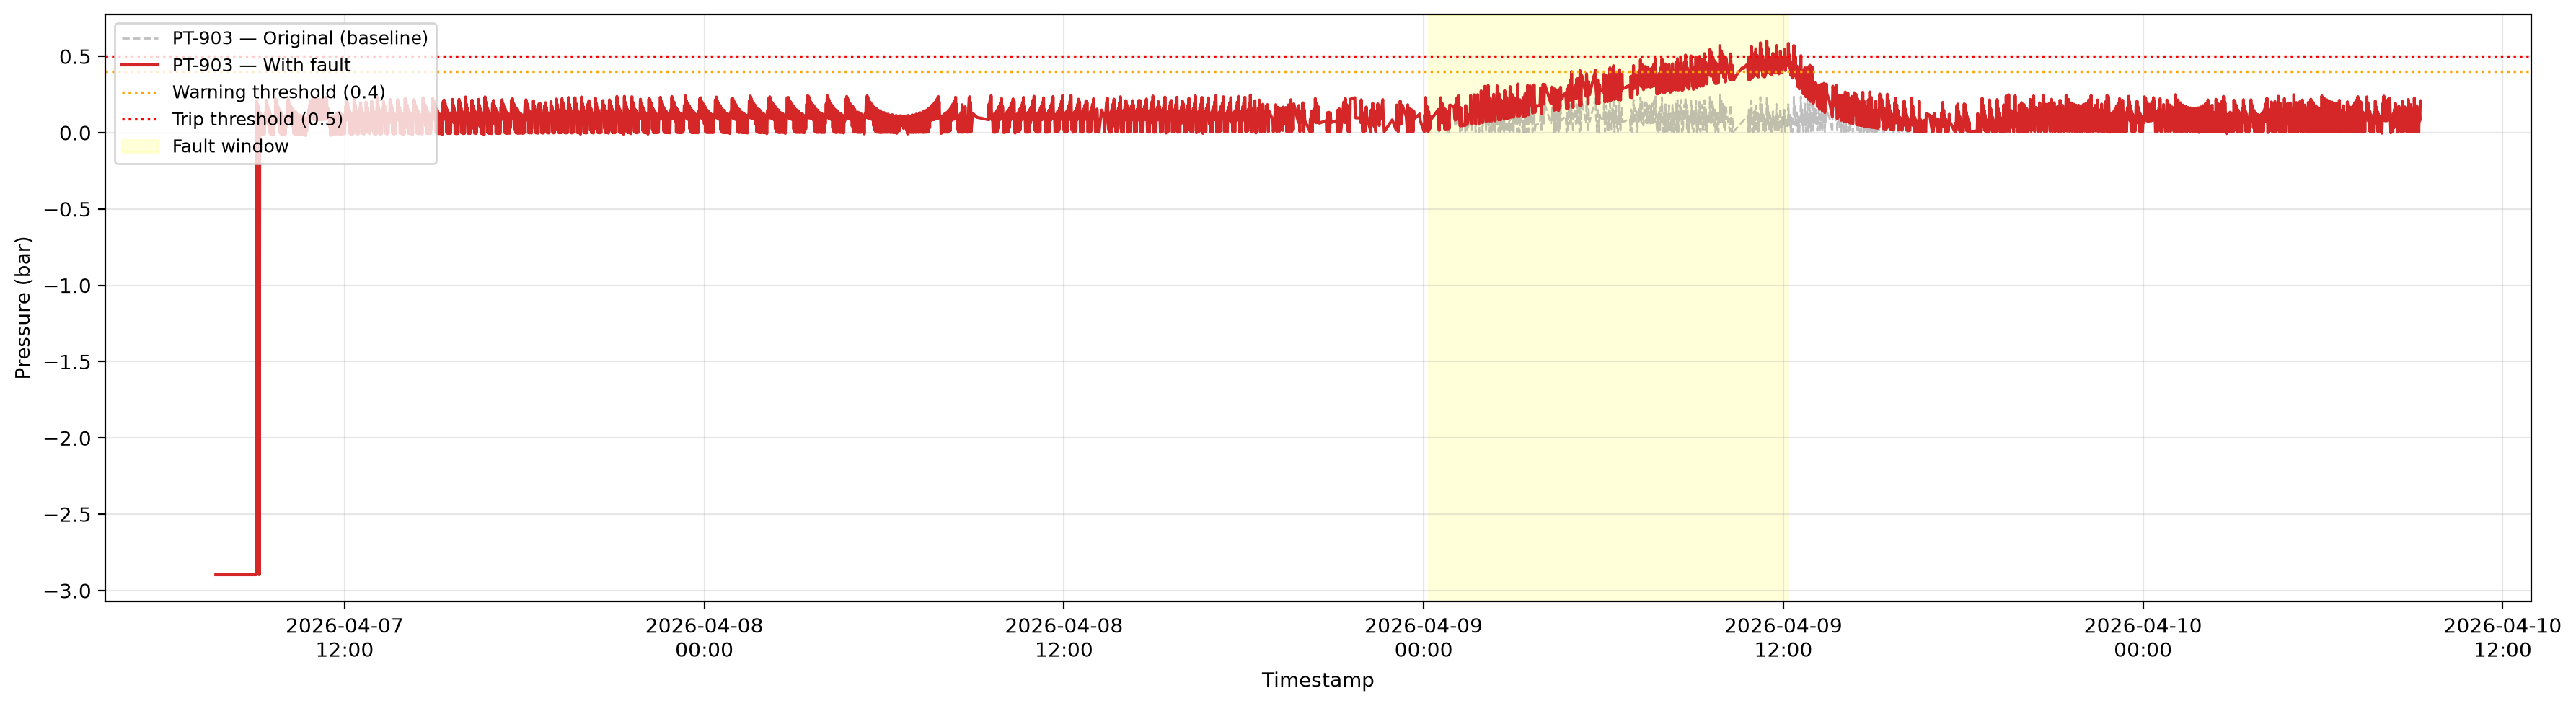
\includegraphics[width=0.95\textwidth]{imgs/fault_f1_severe_s17.png}
    \caption{F1 (clogged exhaust filters), severe severity, Session 17: PT-903 with and without the injected fault. The fault lasts 12 hours, starting 55\% of the way through the session.}
    \label{fig:ap2_f1_severe_s17}
\end{figure}

\begin{figure}[htbp]
    \centering
    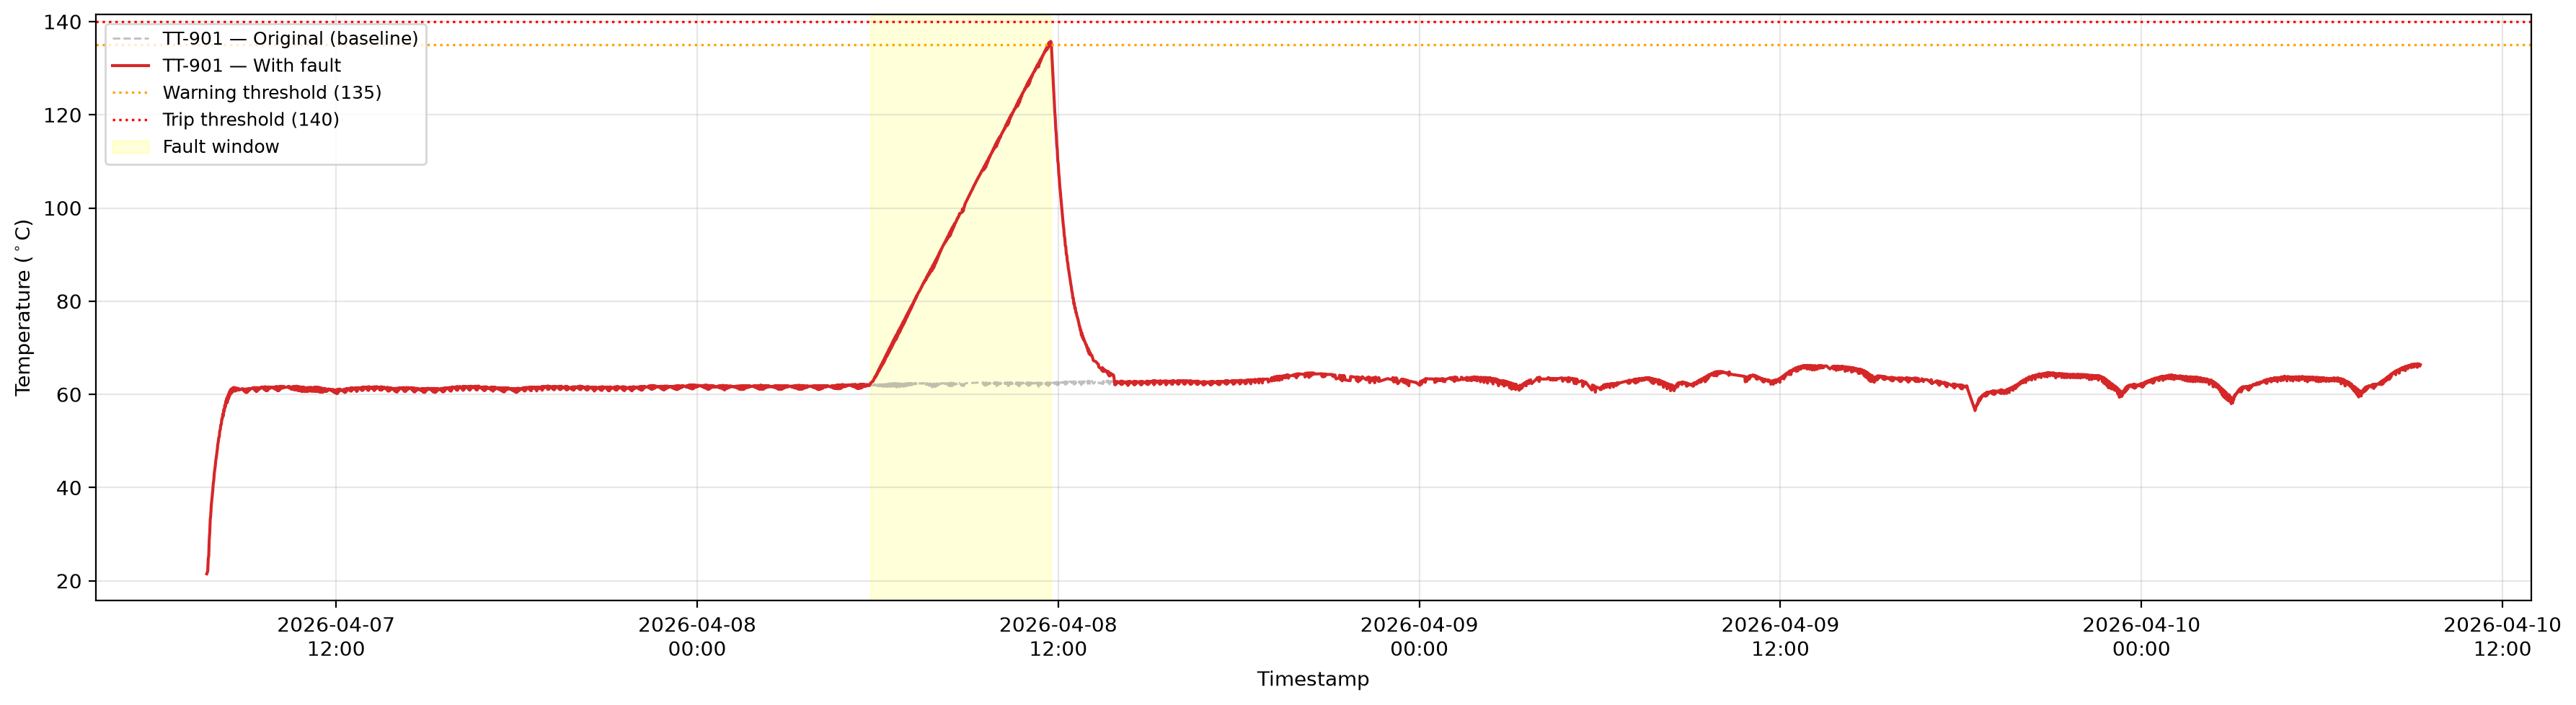
\includegraphics[width=0.95\textwidth]{imgs/fault_f2_small_s17.png}
    \caption{F2 (insufficient cooling), small severity, Session 17: TT-901 with and without the injected fault. The fault lasts 6 hours, starting 30\% of the way through the session.}
    \label{fig:ap2_f2_small_s17}
\end{figure}

\begin{figure}[htbp]
    \centering
    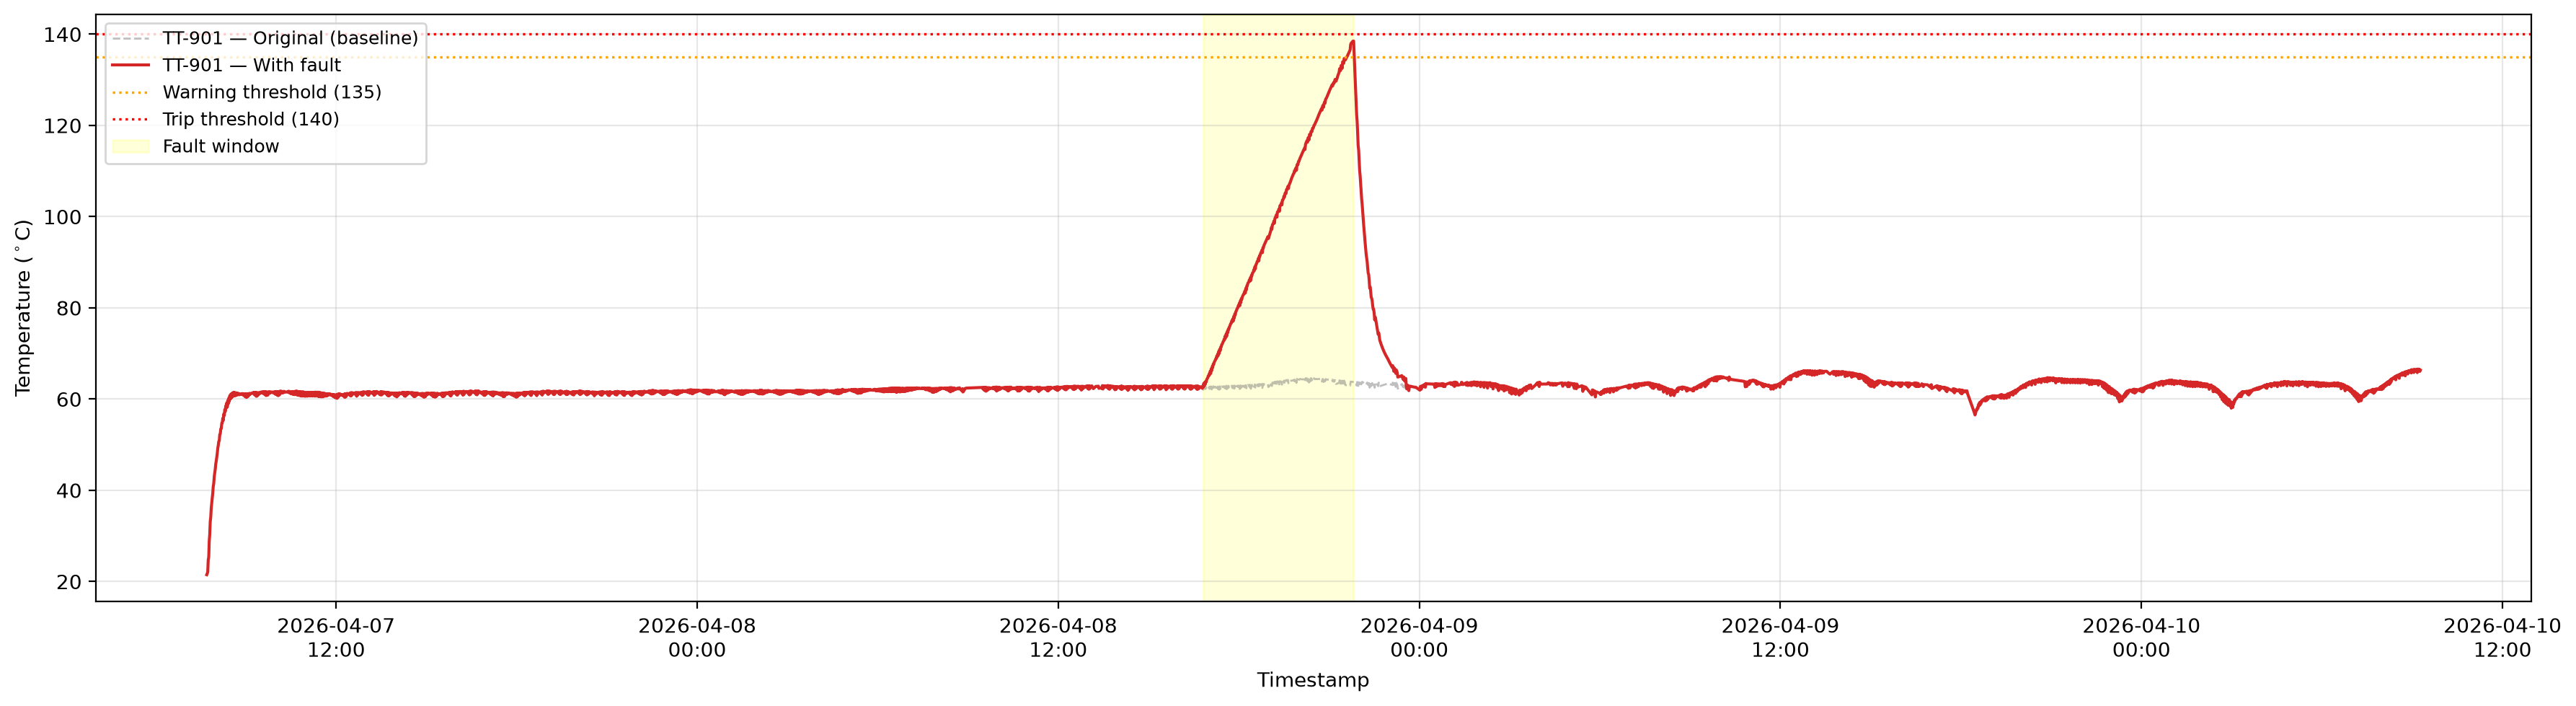
\includegraphics[width=0.95\textwidth]{imgs/fault_f2_medium_s17.png}
    \caption{F2 (insufficient cooling), medium severity, Session 17: TT-901 with and without the injected fault. The fault lasts 5 hours, starting 45\% of the way through the session.}
    \label{fig:ap2_f2_medium_s17}
\end{figure}

\begin{figure}[htbp]
    \centering
    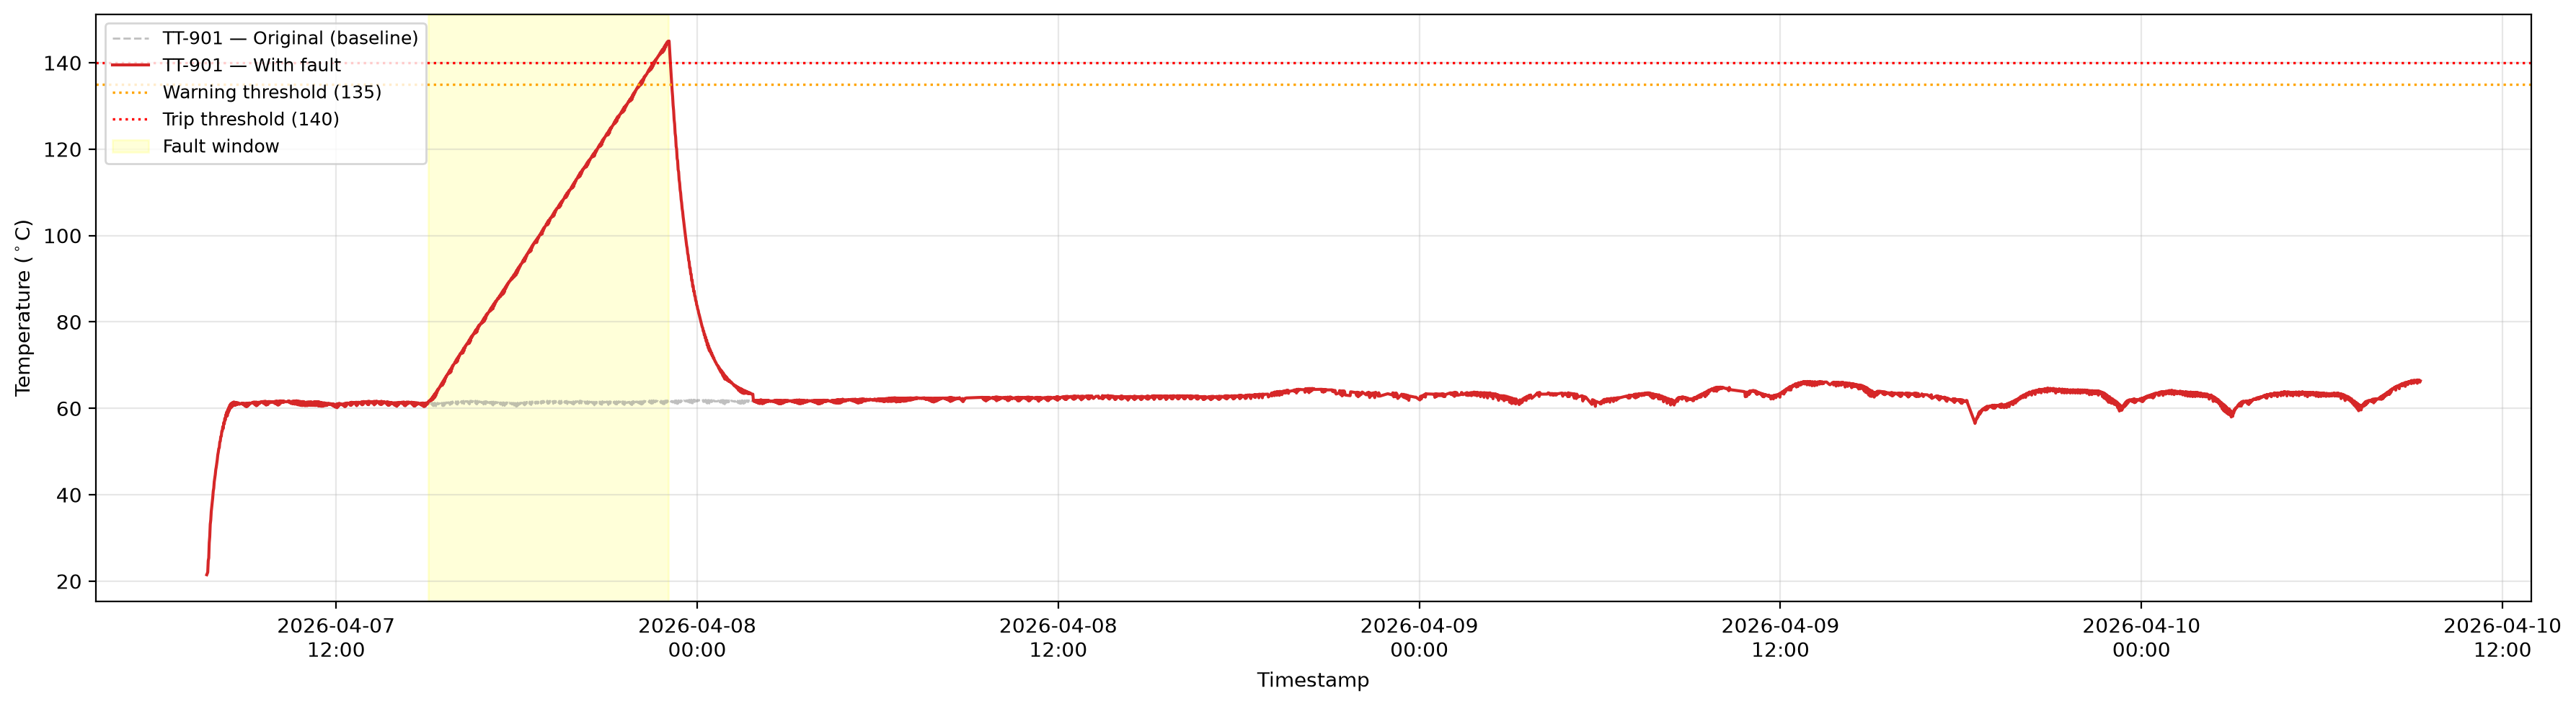
\includegraphics[width=0.95\textwidth]{imgs/fault_f2_severe_s17.png}
    \caption{F2 (insufficient cooling), severe severity, Session 17: TT-901 with and without the injected fault. The fault lasts 8 hours, starting 10\% of the way through the session.}
    \label{fig:ap2_f2_severe_s17}
\end{figure}

\begin{figure}[htbp]
    \centering
    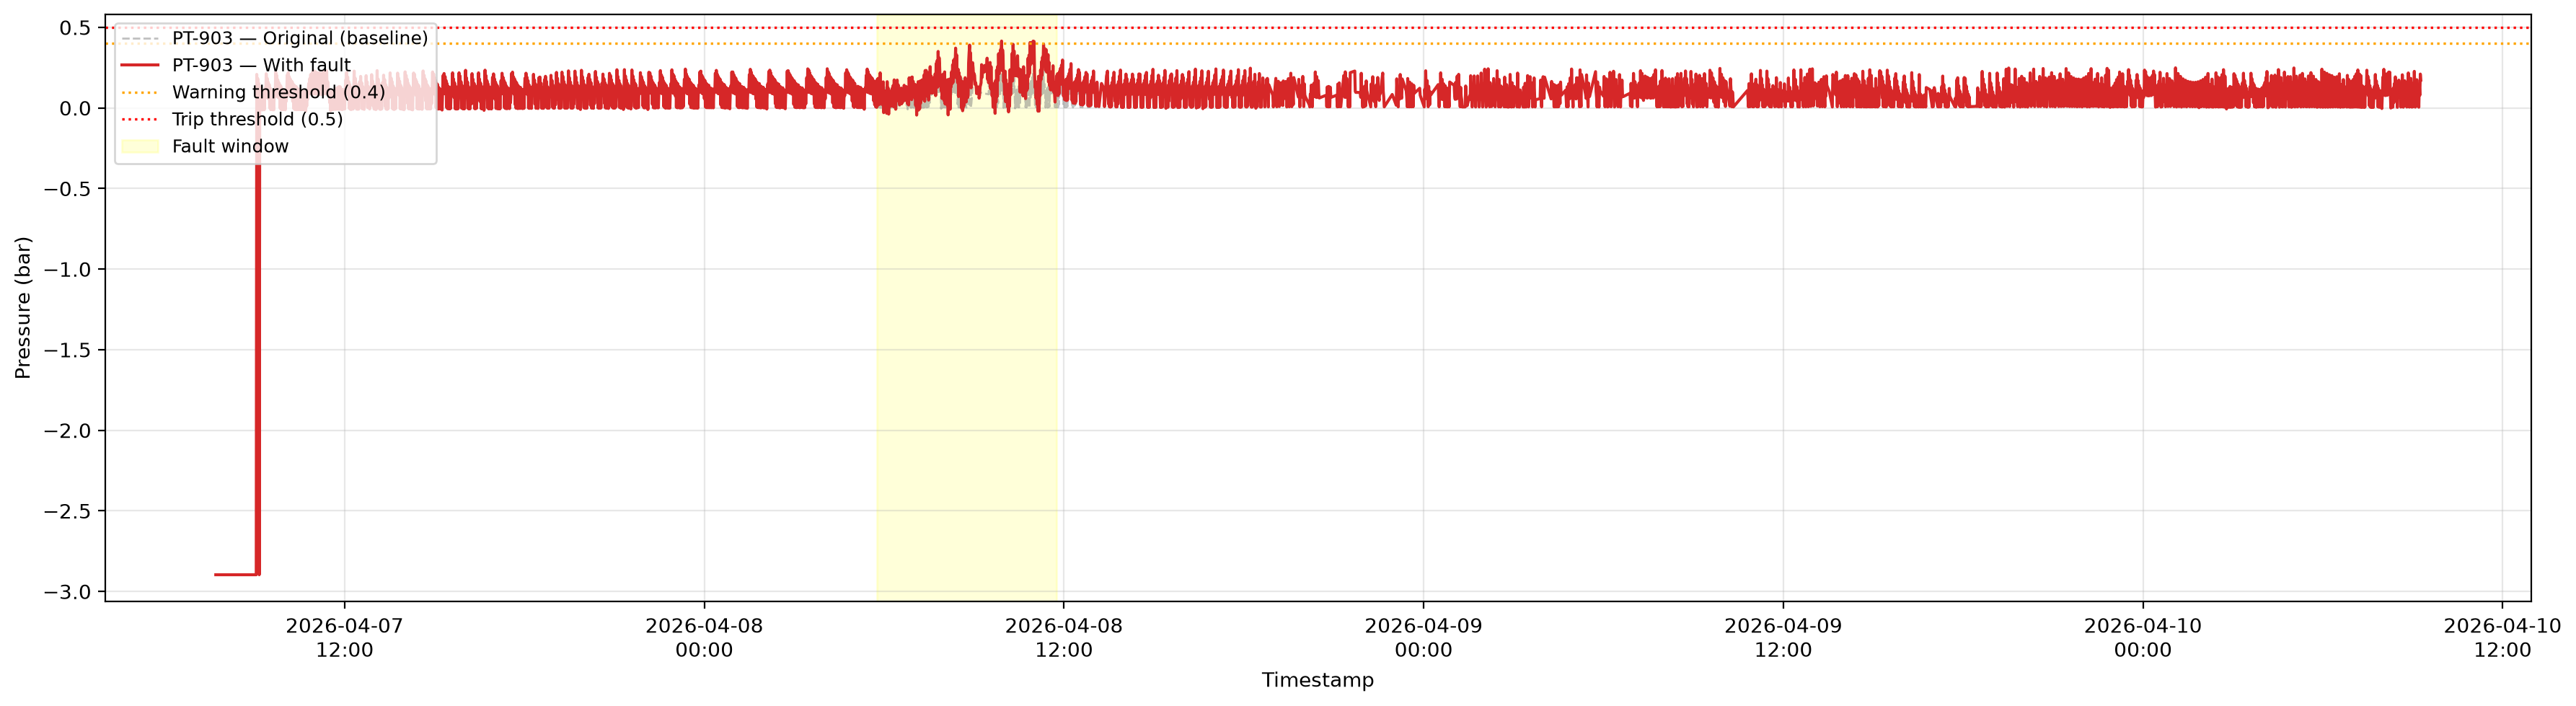
\includegraphics[width=0.95\textwidth]{imgs/fault_f3_small_s17.png}
    \caption{F3 (float valve fault), small severity, Session 17: PT-903 with and without the injected fault. The fault lasts 6 hours, starting 30\% of the way through the session.}
    \label{fig:ap2_f3_small_s17}
\end{figure}

\begin{figure}[htbp]
    \centering
    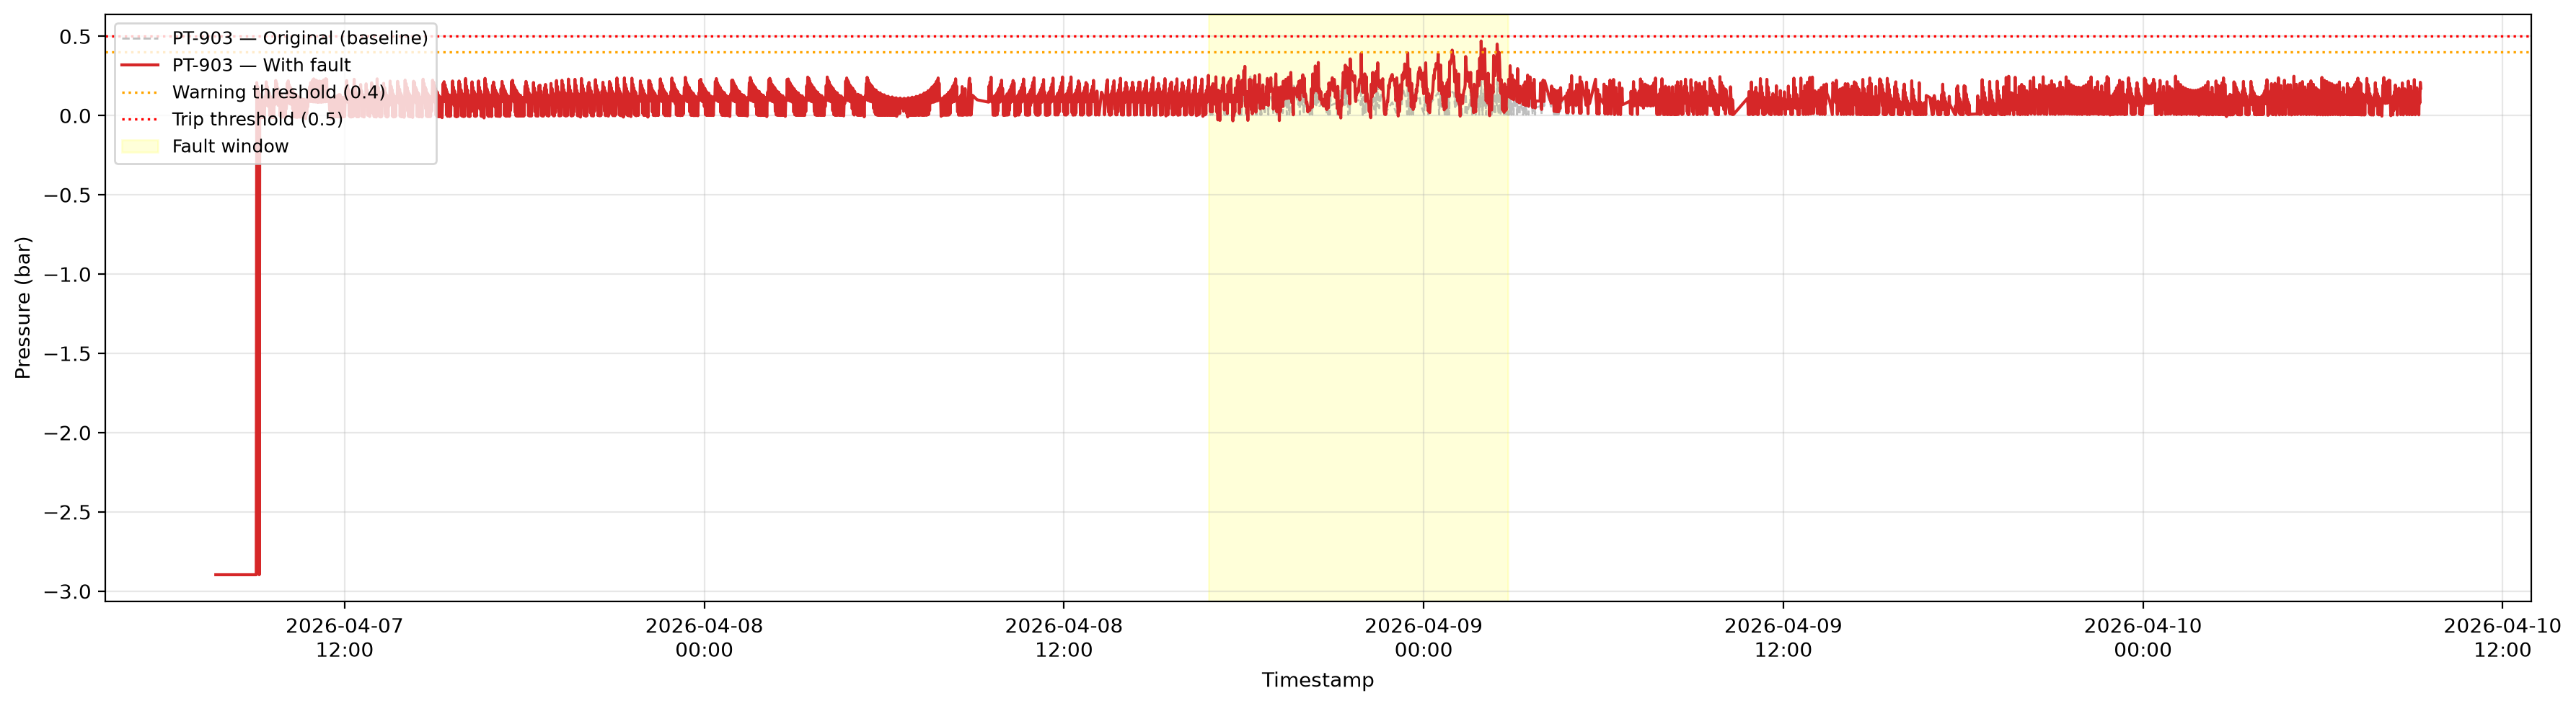
\includegraphics[width=0.95\textwidth]{imgs/fault_f3_medium_s17.png}
    \caption{F3 (float valve fault), medium severity, Session 17: PT-903 with and without the injected fault. The fault lasts 10 hours, starting 45\% of the way through the session.}
    \label{fig:ap2_f3_medium_s17}
\end{figure}

\begin{figure}[htbp]
    \centering
    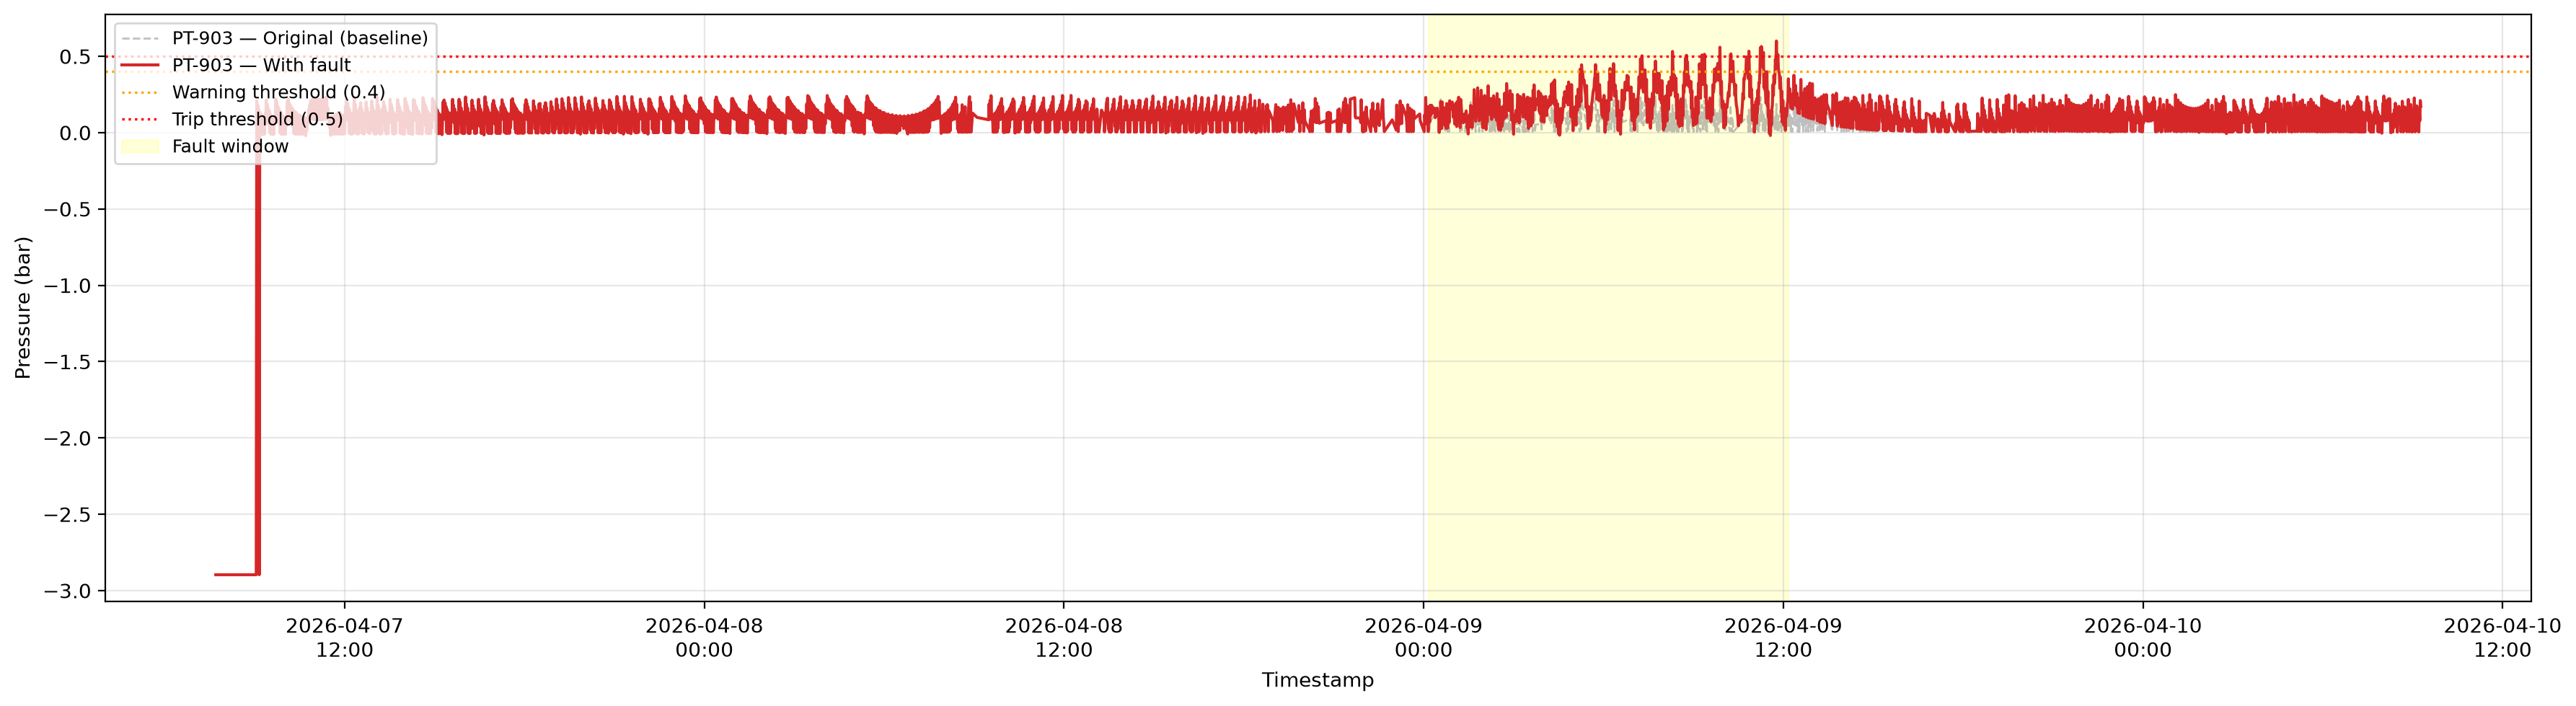
\includegraphics[width=0.95\textwidth]{imgs/fault_f3_severe_s17.png}
    \caption{F3 (float valve fault), severe severity, Session 17: PT-903 with and without the injected fault. The fault lasts 12 hours, starting 55\% of the way through the session.}
    \label{fig:ap2_f3_severe_s17}
\end{figure}

\begin{figure}[htbp]
    \centering
    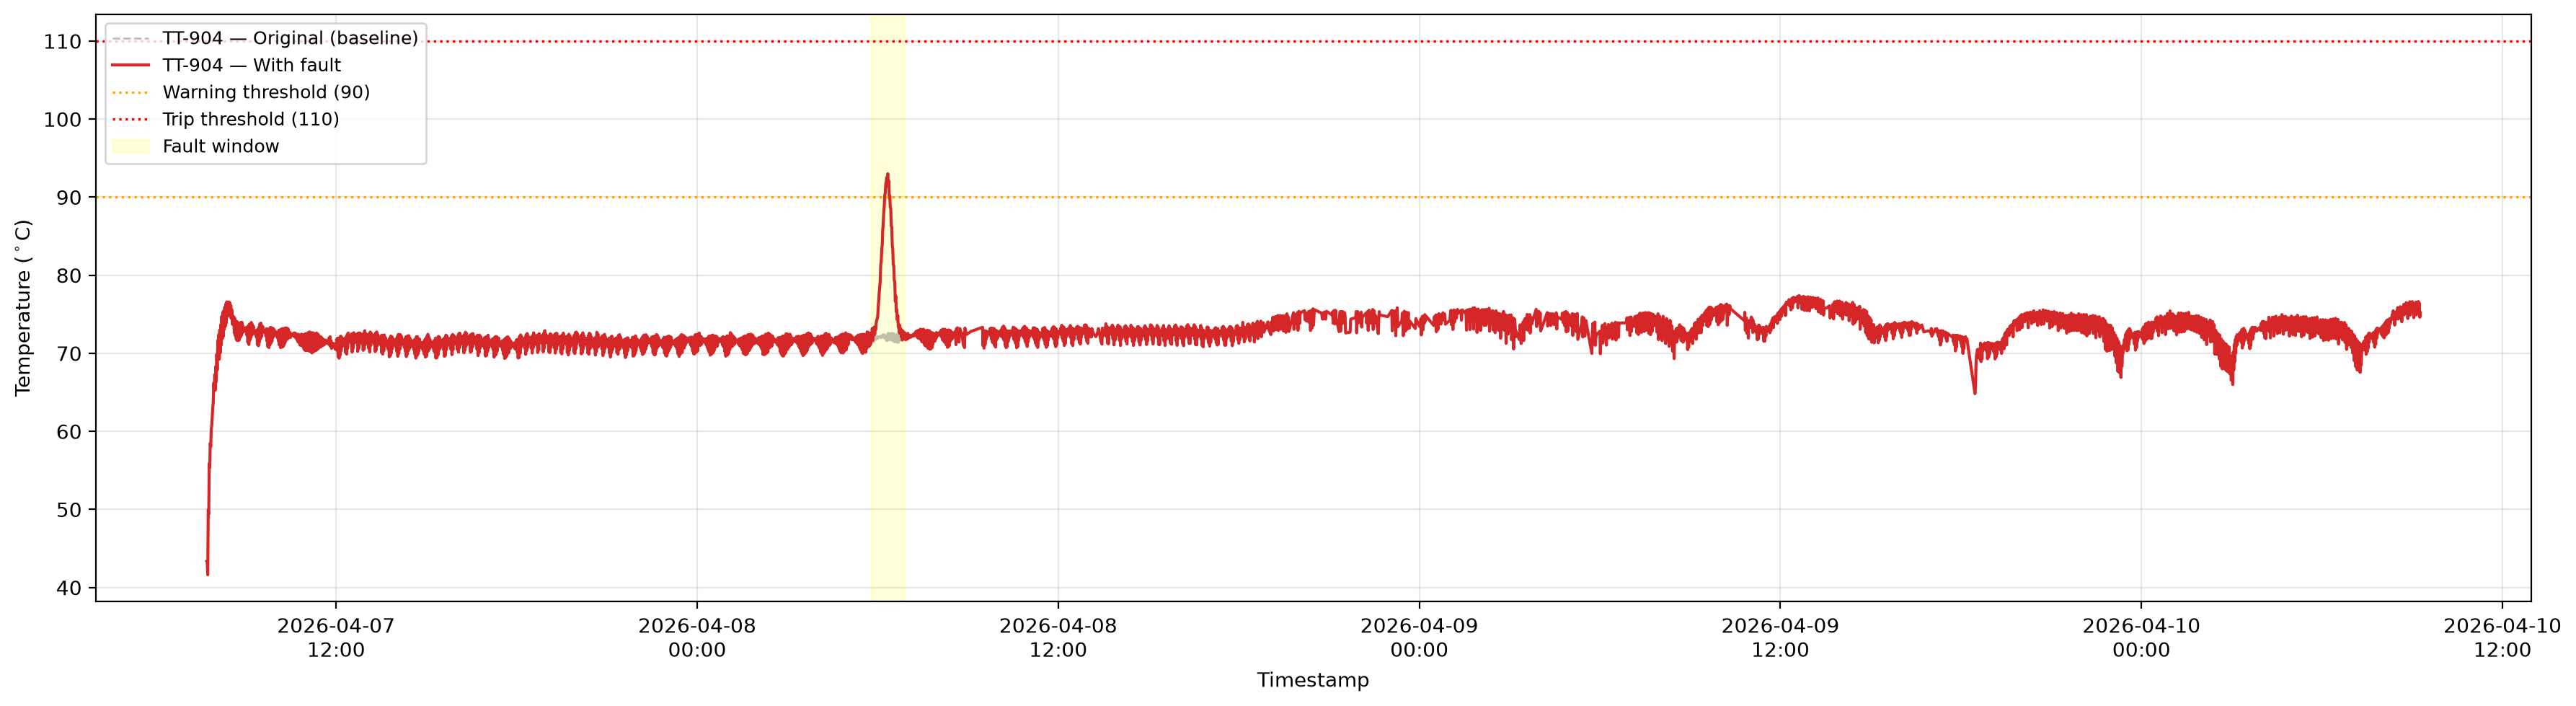
\includegraphics[width=0.95\textwidth]{imgs/fault_f4_small_s17.png}
    \caption{F4 (defective bearing), small severity, Session 17: TT-904 with and without the injected fault. The fault lasts 67 minutes, starting 30\% of the way through the session.}
    \label{fig:ap2_f4_small_s17}
\end{figure}

\begin{figure}[htbp]
    \centering
    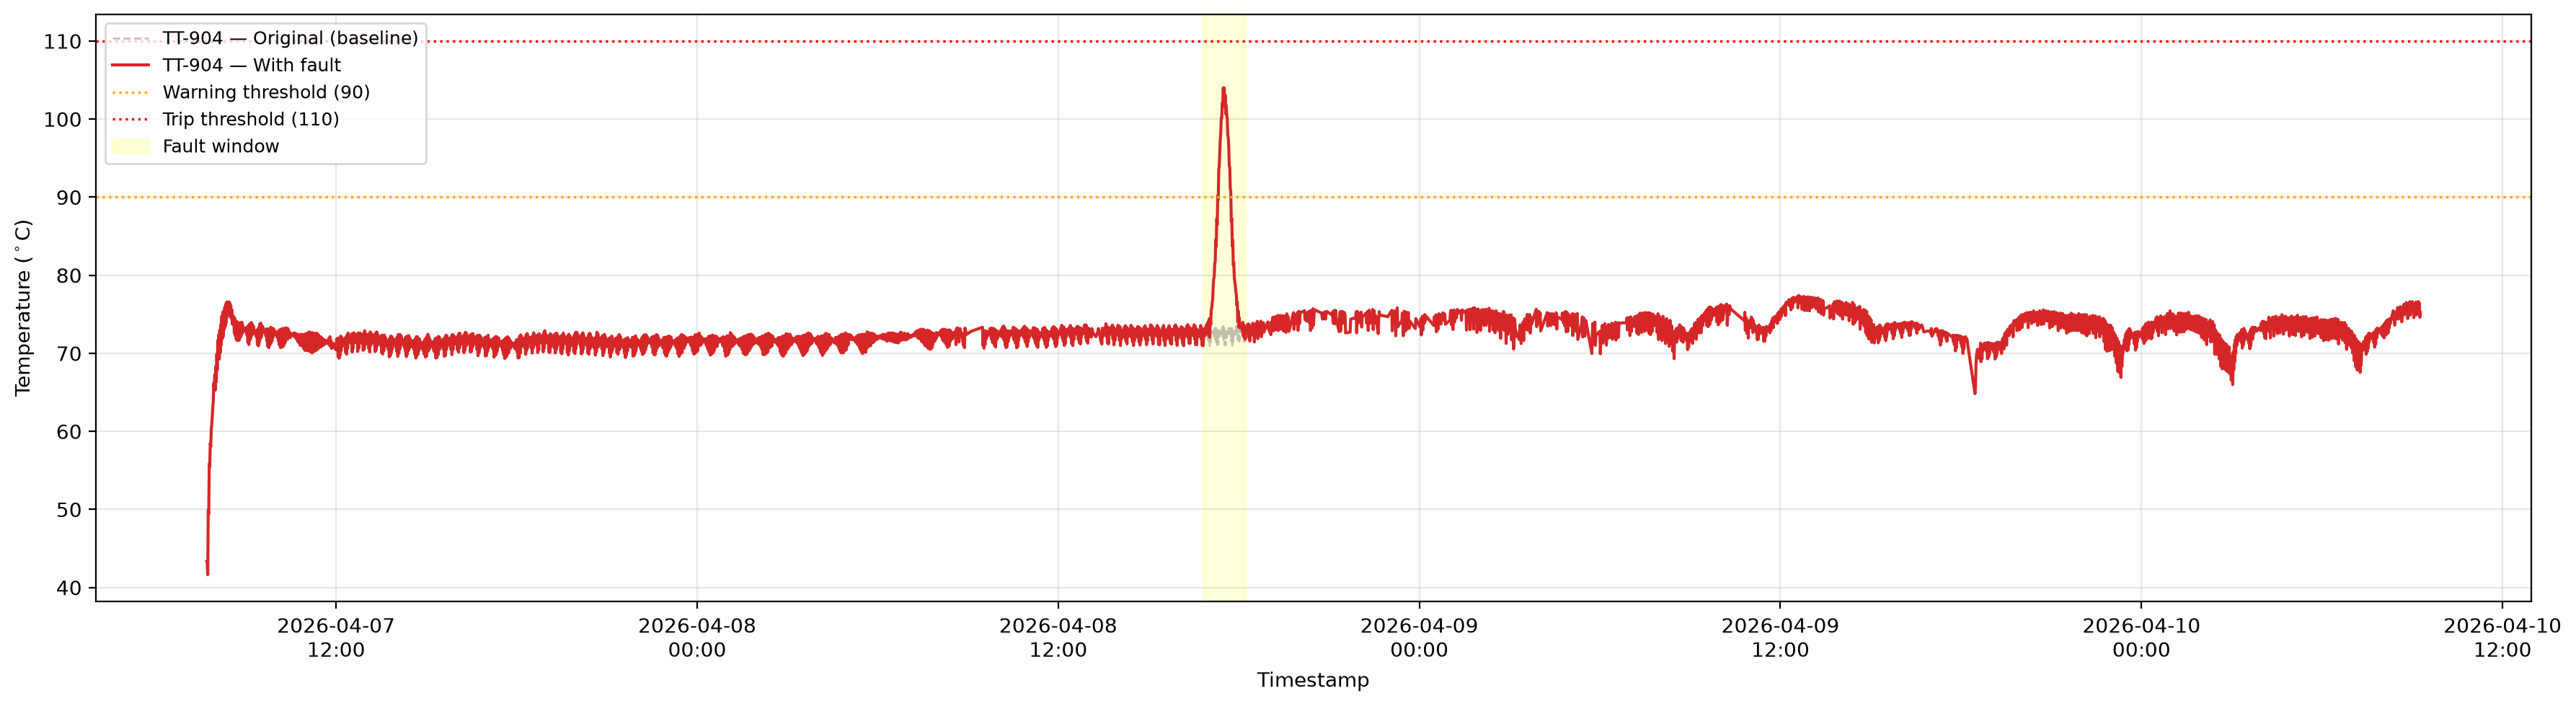
\includegraphics[width=0.95\textwidth]{imgs/fault_f4_medium_s17.png}
    \caption{F4 (defective bearing), medium severity, Session 17: TT-904 with and without the injected fault. The fault lasts 84 minutes, starting 45\% of the way through the session.}
    \label{fig:ap2_f4_medium_s17}
\end{figure}

\begin{figure}[htbp]
    \centering
    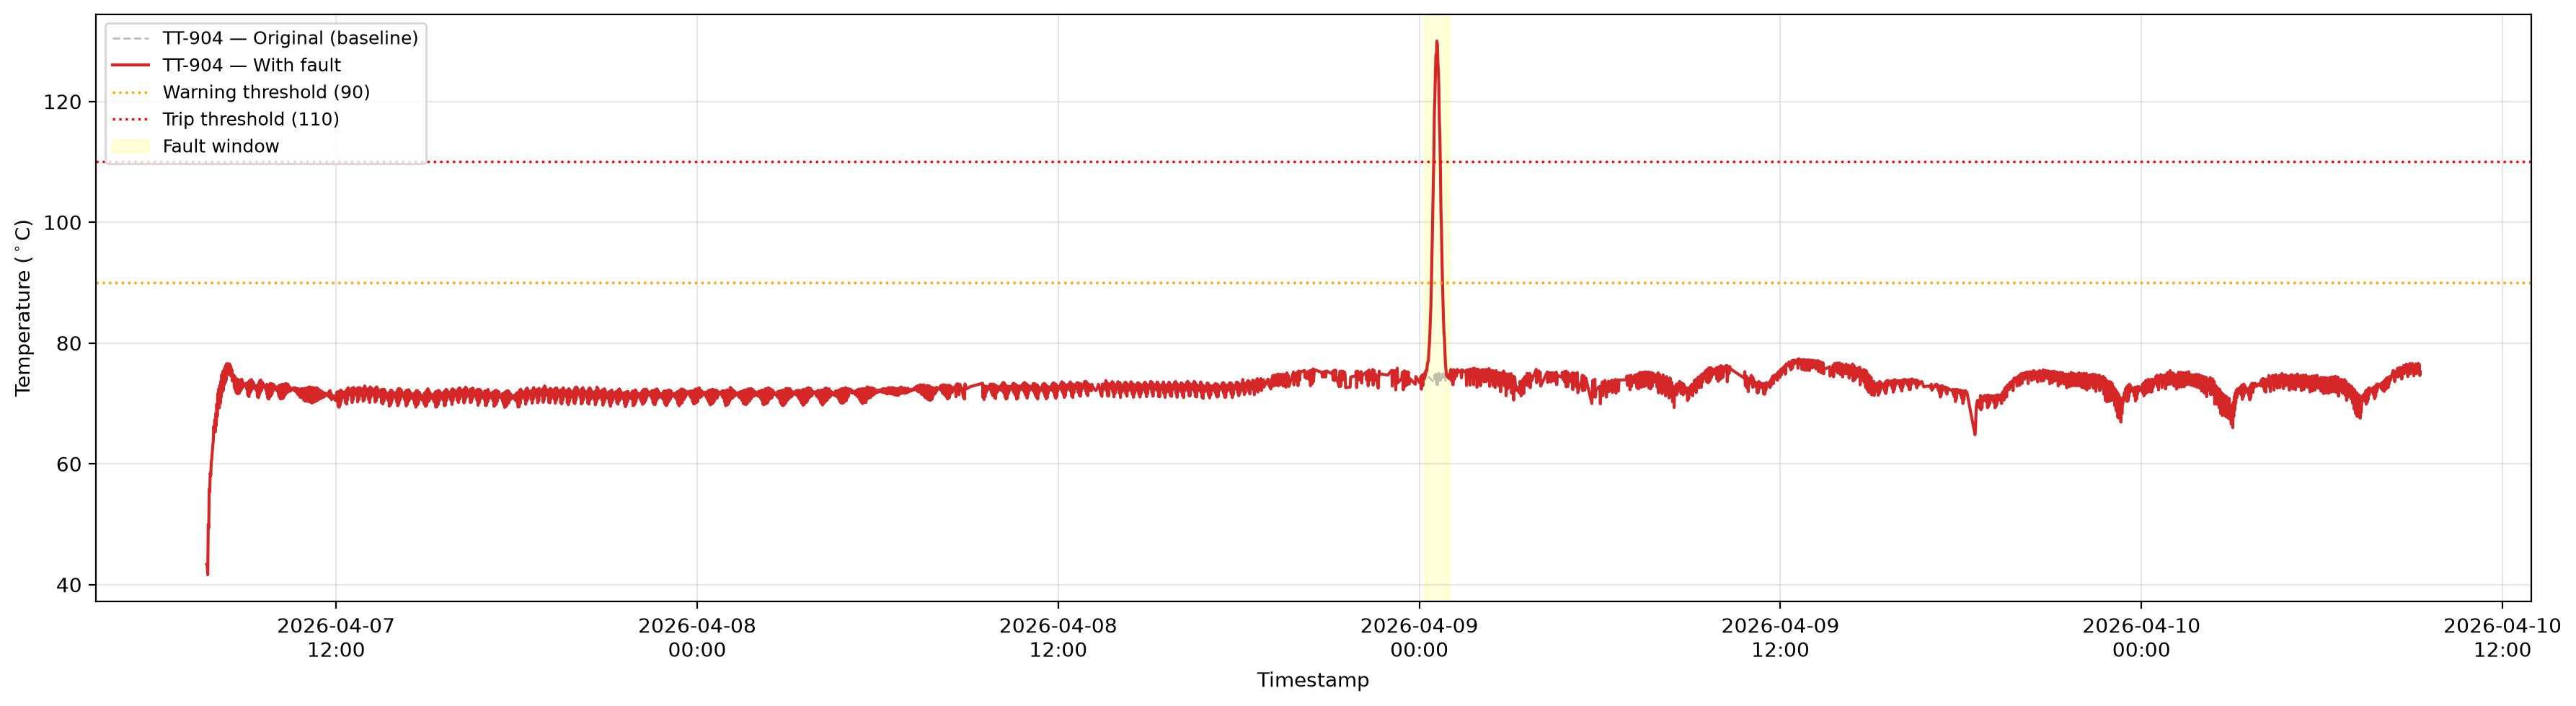
\includegraphics[width=0.95\textwidth]{imgs/fault_f4_severe_s17.png}
    \caption{F4 (defective bearing), severe severity, Session 17: TT-904 with and without the injected fault. The fault lasts 51 minutes, starting 55\% of the way through the session.}
    \label{fig:ap2_f4_severe_s17}
\end{figure}


\section{Combined Fault Scenarios} \label{app:fault_combined}

Combo A injects F1 at severe severity and F3 at small severity, both acting on PT-903, with the two windows
partially overlapping. A single panel therefore suffices. Combo B injects F2 at medium severity on TT-901
and F4 at severe severity on TT-904, with the F4 window fully contained within the longer F2 window; both
sensors are shown, and both component windows are shaded in each panel so that the timing relationship
between the two faults remains visible in either one.

\begin{figure}[htbp]
    \centering
    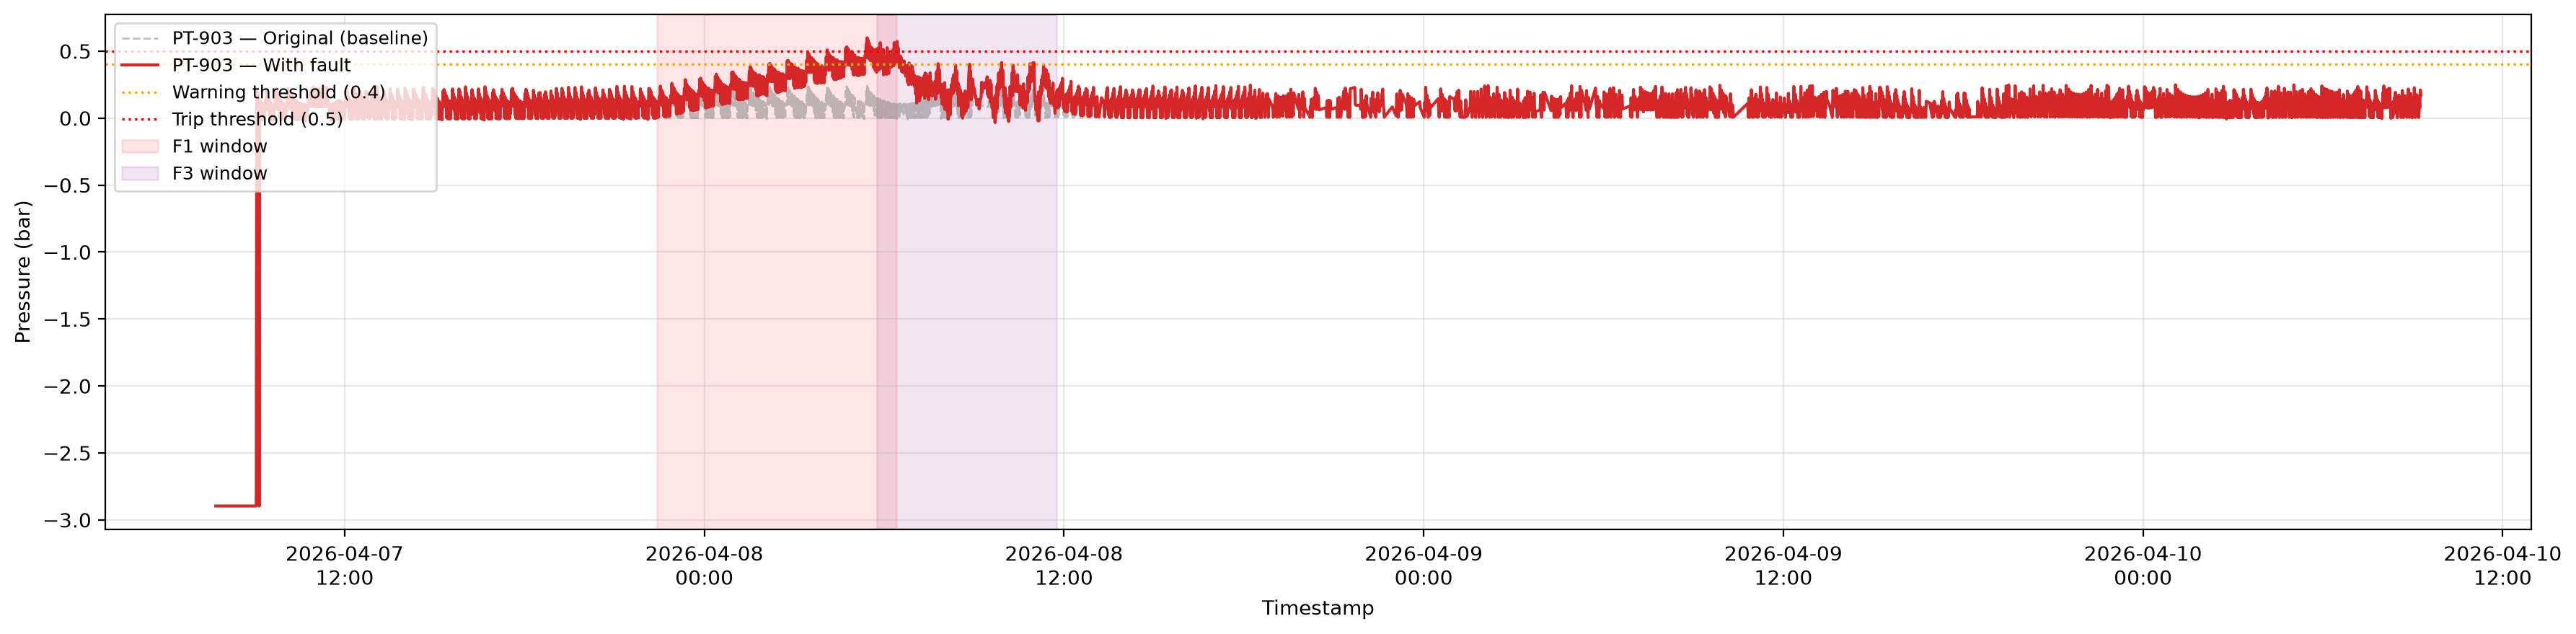
\includegraphics[width=0.95\textwidth]{imgs/fault_combo_a_s17.png}
    \caption{Combo A (F1 severe + F3 small), Session 17: PT-903 with and without the injected faults. The overlap between the two windows is shorter than in Session 16.}
    \label{fig:ap2_combo_a_s17}
\end{figure}

\begin{figure}[htbp]
    \centering
    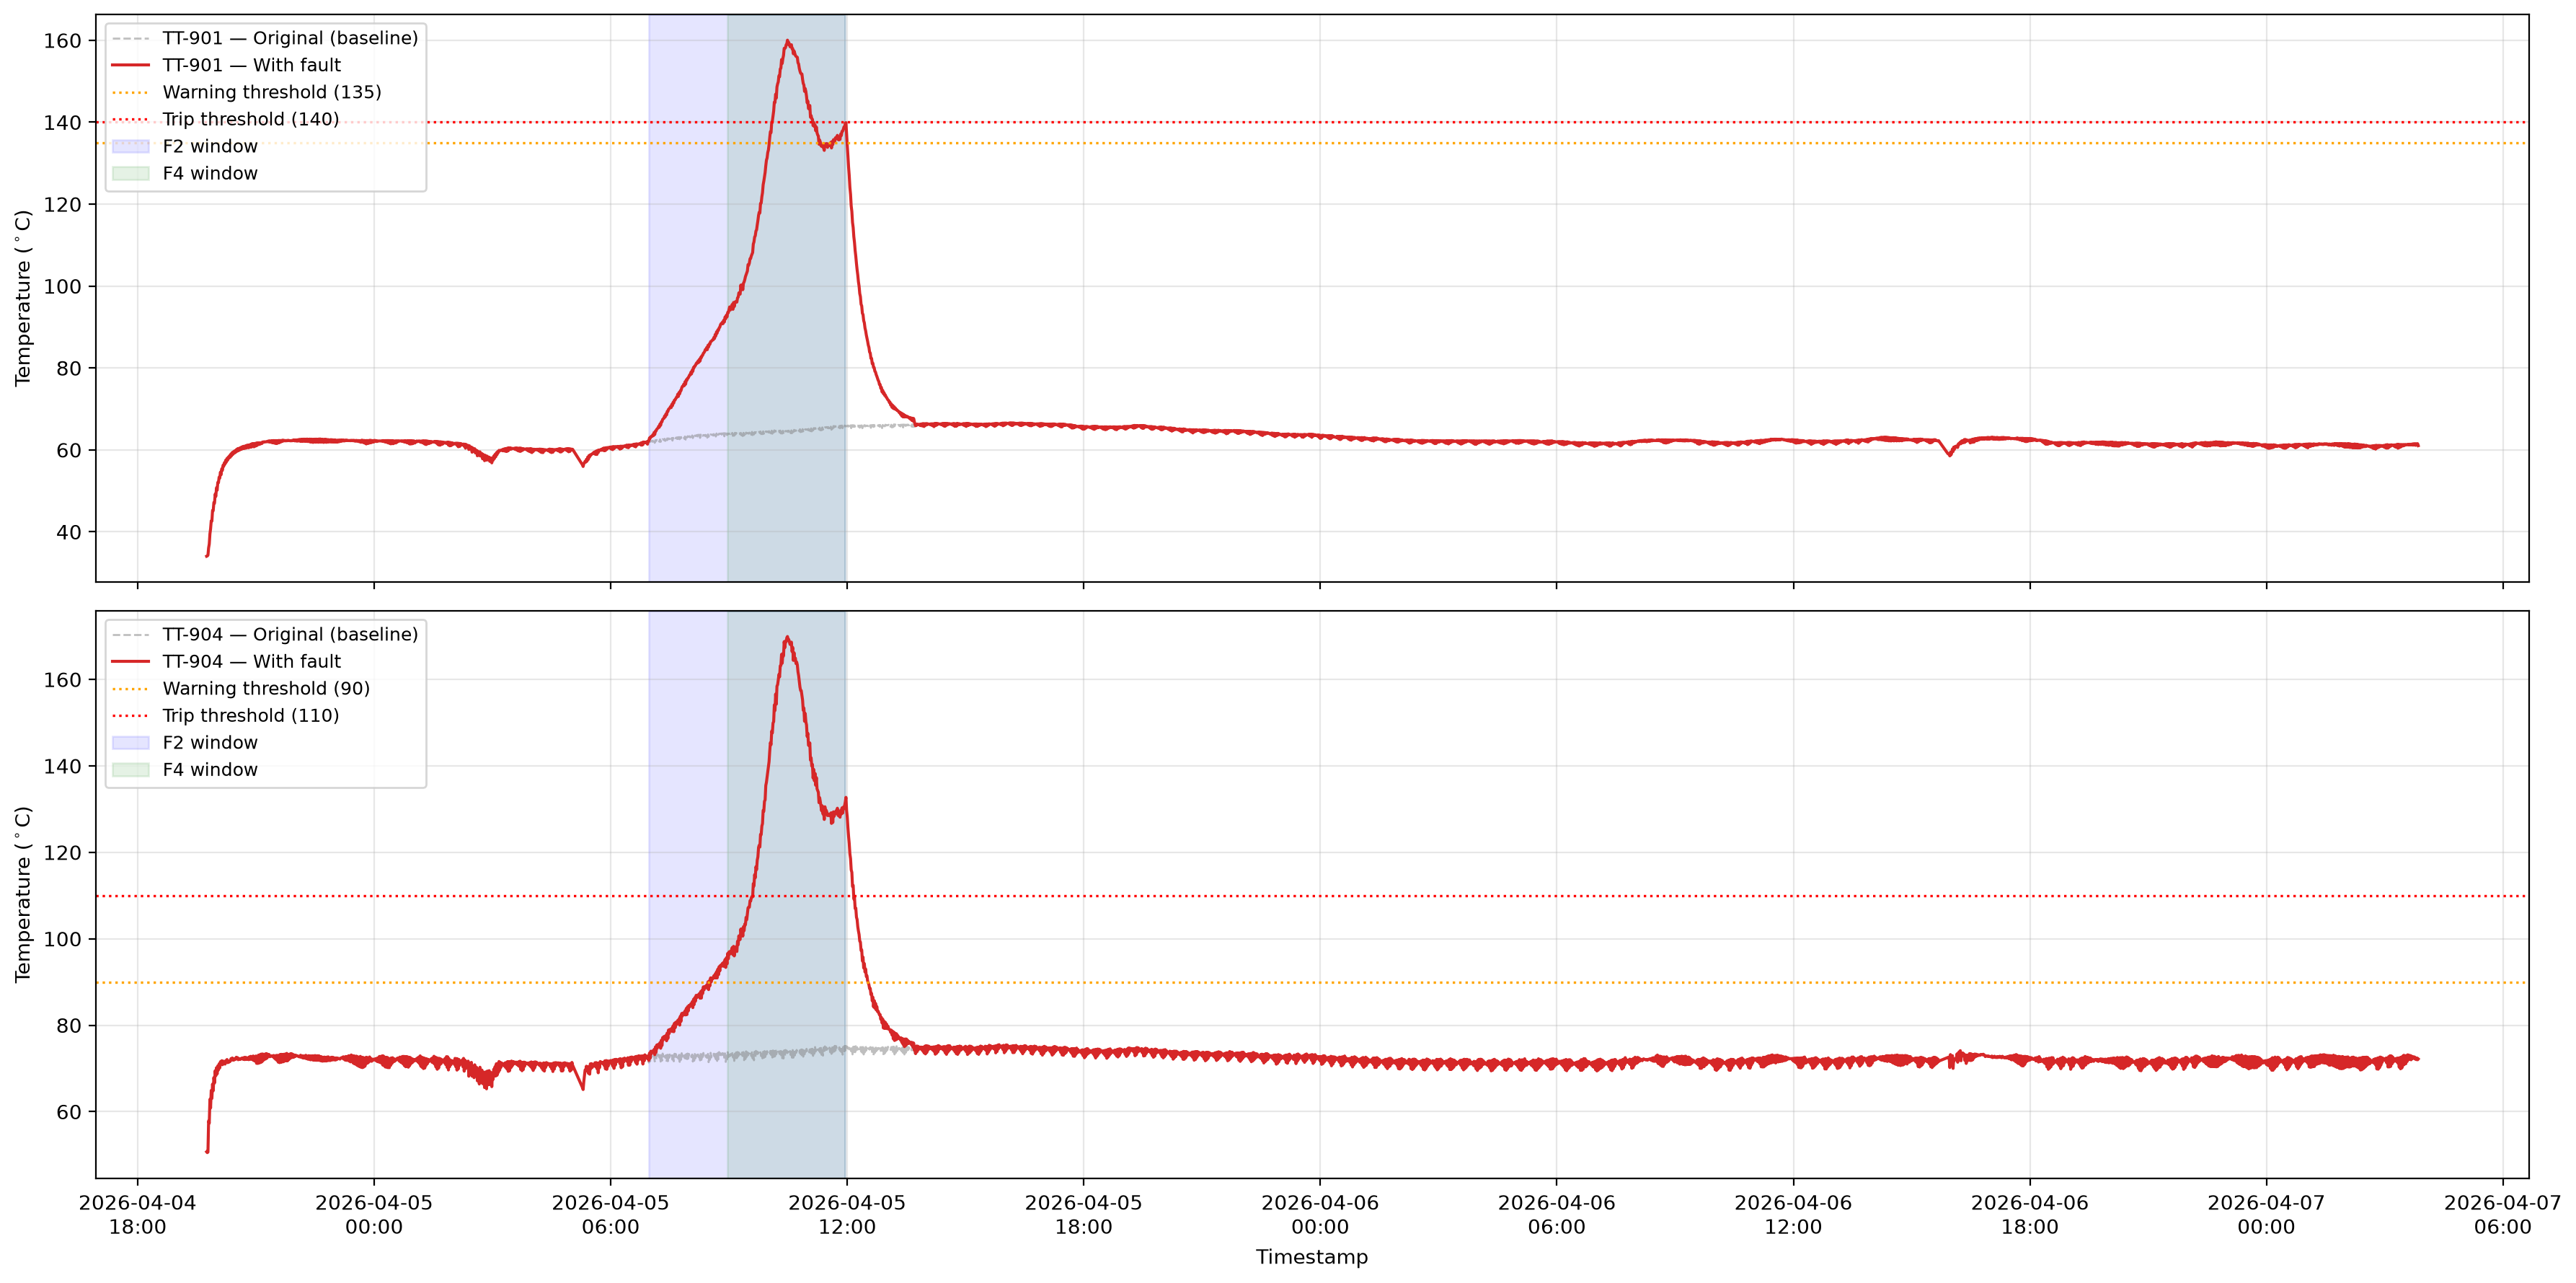
\includegraphics[width=0.95\textwidth]{imgs/fault_combo_b_s16.png}
    \caption{Combo B (F2 medium + F4 severe), Session 16: TT-901 (top) and TT-904 (bottom) with and without the injected faults. The F4 spike on TT-904 occurs entirely within the F2 window on TT-901.}
    \label{fig:ap2_combo_b_s16}
\end{figure}

\begin{figure}[htbp]
    \centering
    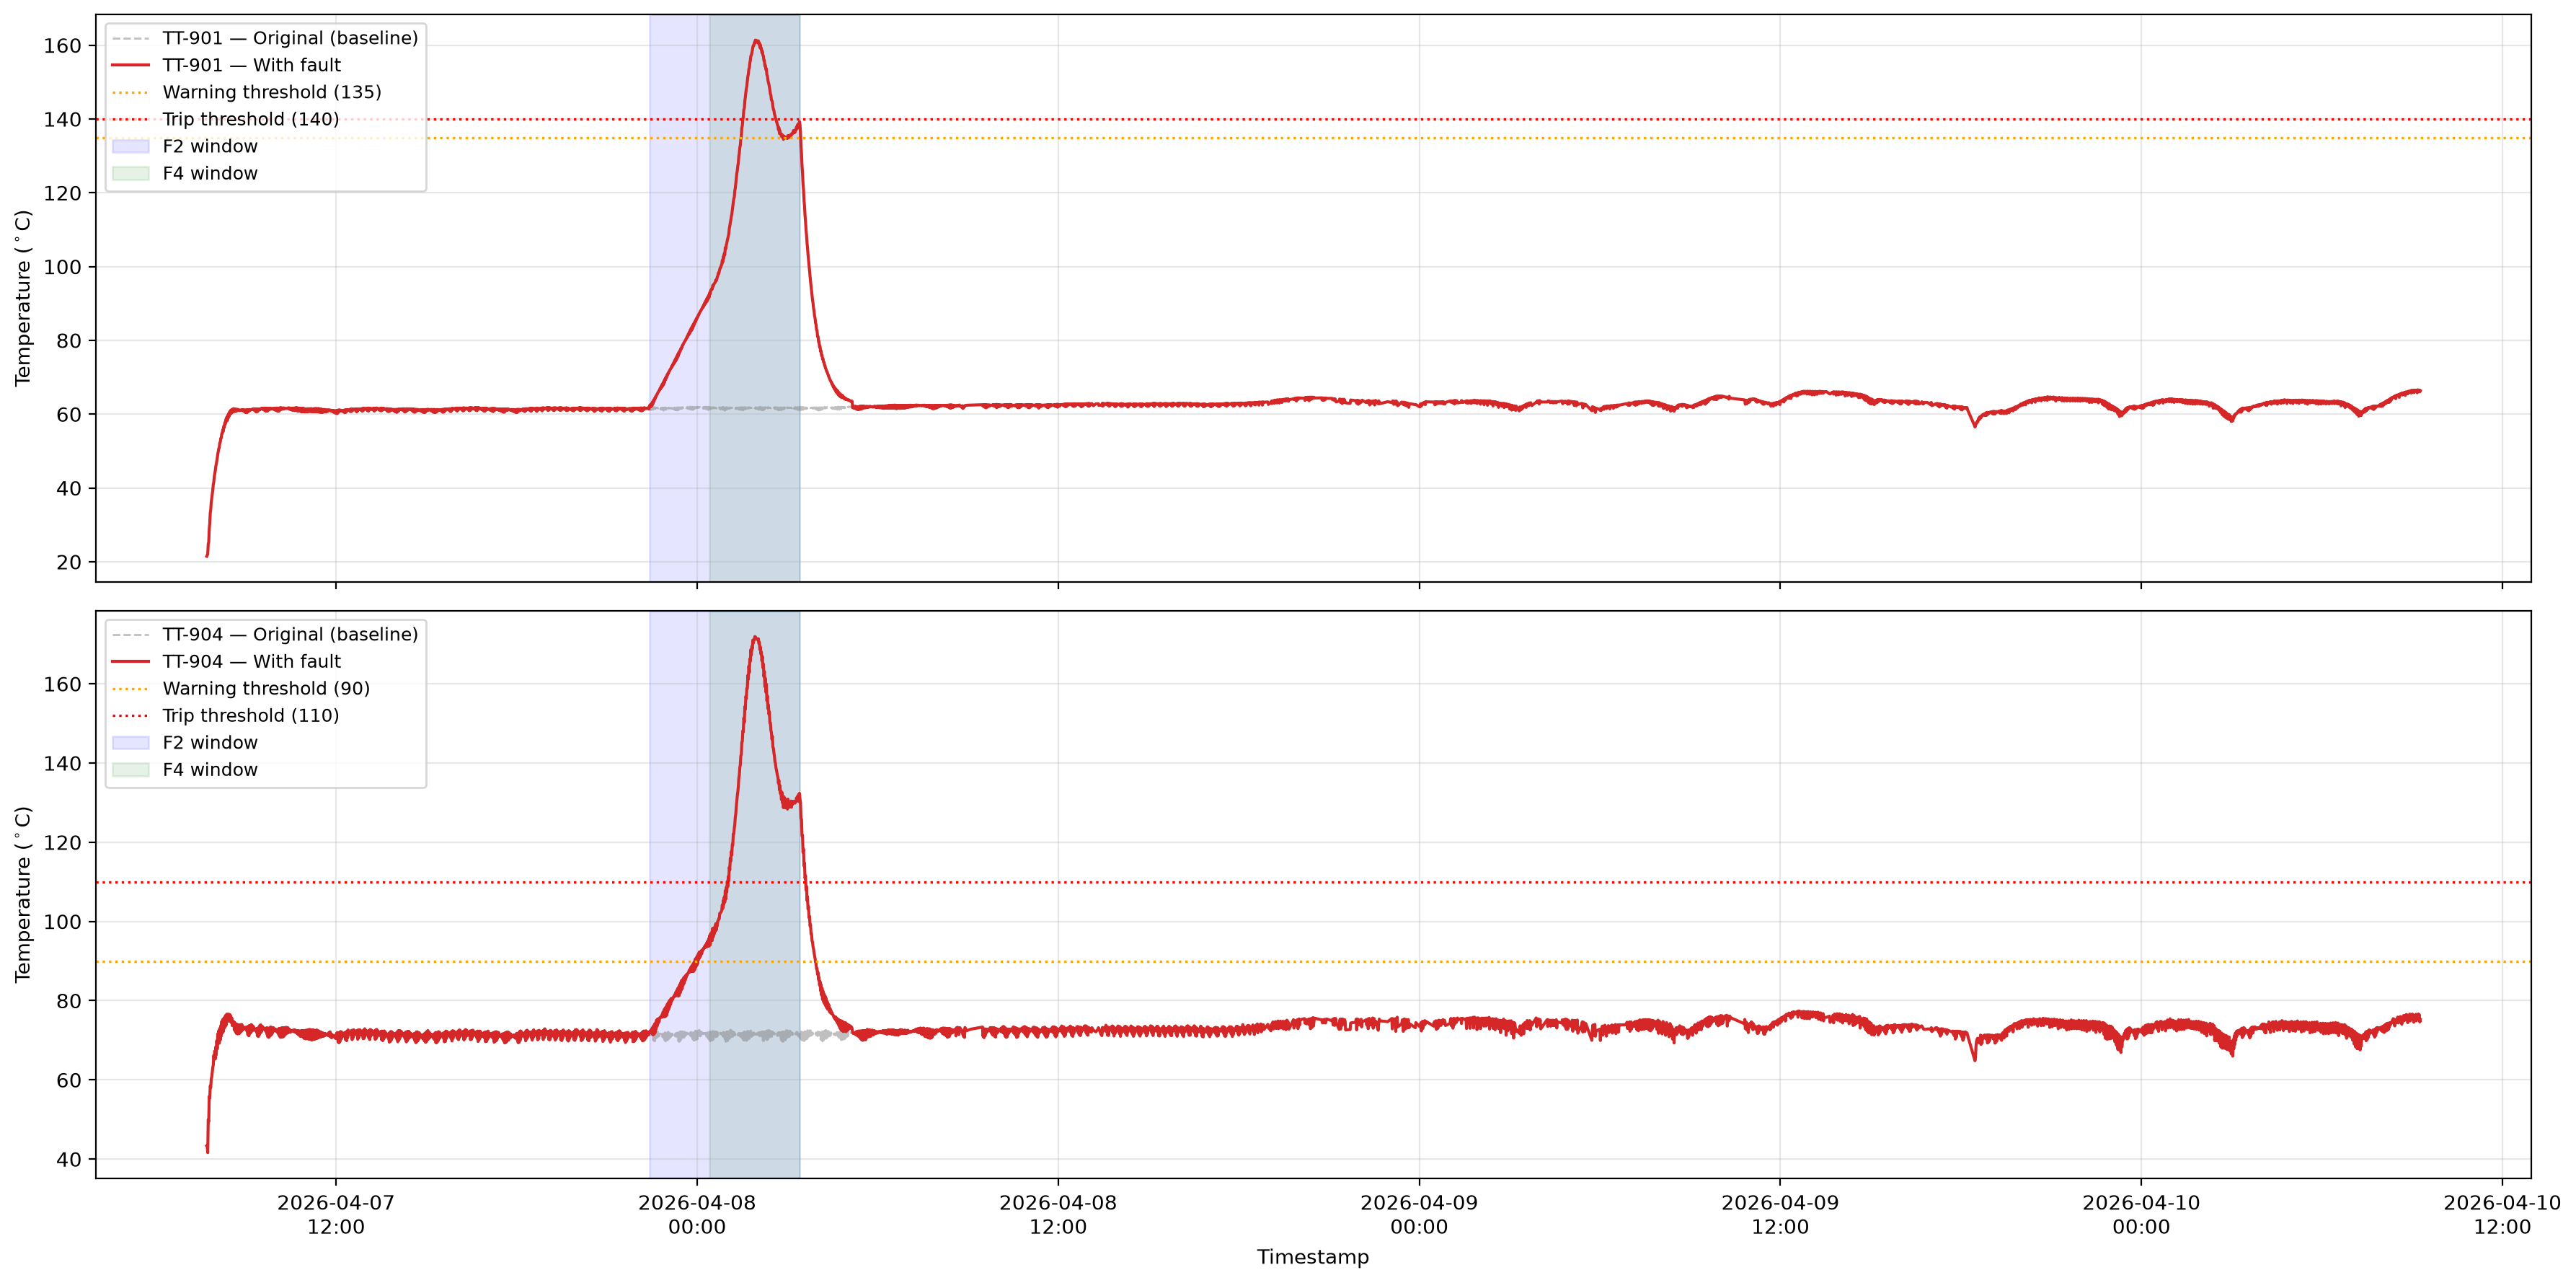
\includegraphics[width=0.95\textwidth]{imgs/fault_combo_b_s17.png}
    \caption{Combo B (F2 medium + F4 severe), Session 17: TT-901 (top) and TT-904 (bottom) with and without the injected faults. The F4 spike on TT-904 occurs entirely within the F2 window on TT-901.}
    \label{fig:ap2_combo_b_s17}
\end{figure}


\section{False Positive Scenarios} \label{app:fault_fp}

The false positive scenario injects a brief Gaussian spike into a single sensor during an otherwise normal
period, reaching 80\% of that sensor's trip threshold and lasting twelve minutes. Unlike the fault
scenarios, the deviation is not propagated to any correlated sensor, so the spike appears in isolation,
which is precisely what makes it physically implausible as a genuine process event. These observations are
labelled \texttt{false\_positive} and carry an \texttt{anomaly\_level} of 0, so a model that flags them as
anomalous is producing a false alarm. A different shading colour is used in these two figures to reflect
that the window is not labelled as an anomaly.

A different sensor is used in each session, TT-902 in Session 16 and TT-903 in Session 17, so that the
scenario is not tied to the behaviour of one particular measurement.

\begin{figure}[htbp]
    \centering
    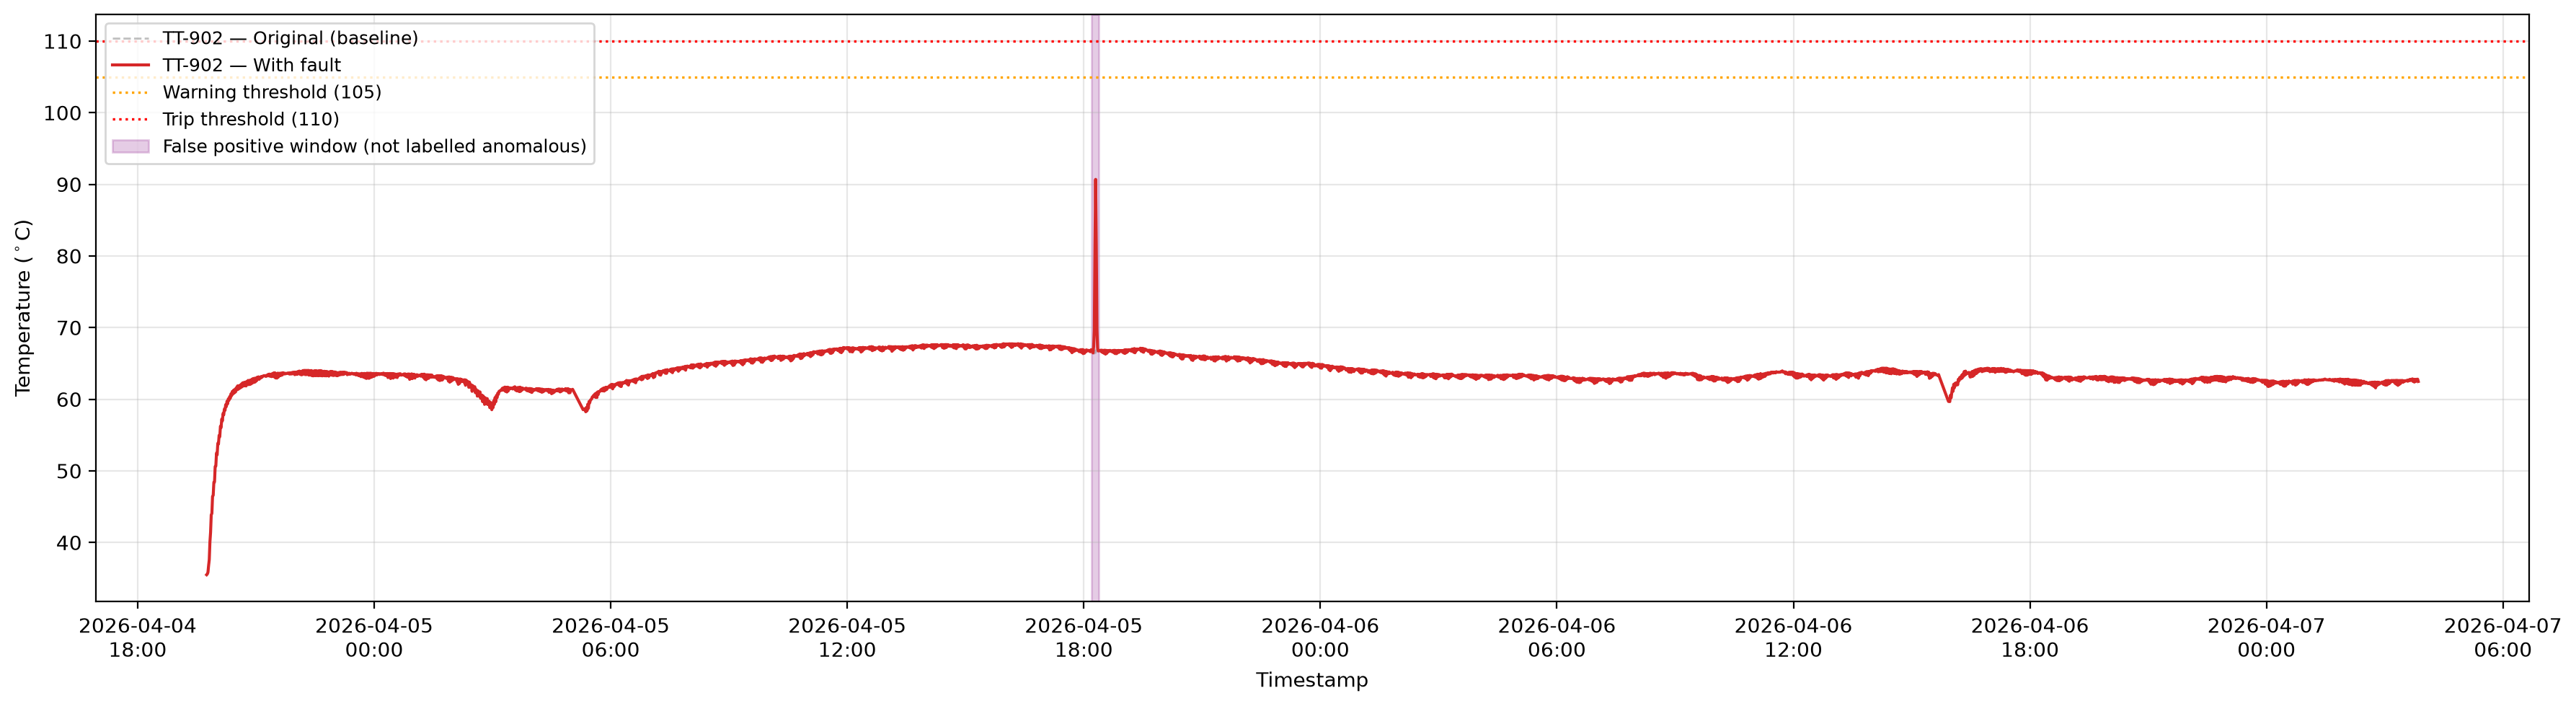
\includegraphics[width=0.95\textwidth]{imgs/fault_fp_s16.png}
    \caption{Standalone false positive scenario, Session 16: TT-902 with and without the injected spike. The spike stays below the trip threshold and is not propagated to any correlated sensor.}
    \label{fig:ap2_fp_s16}
\end{figure}

\begin{figure}[htbp]
    \centering
    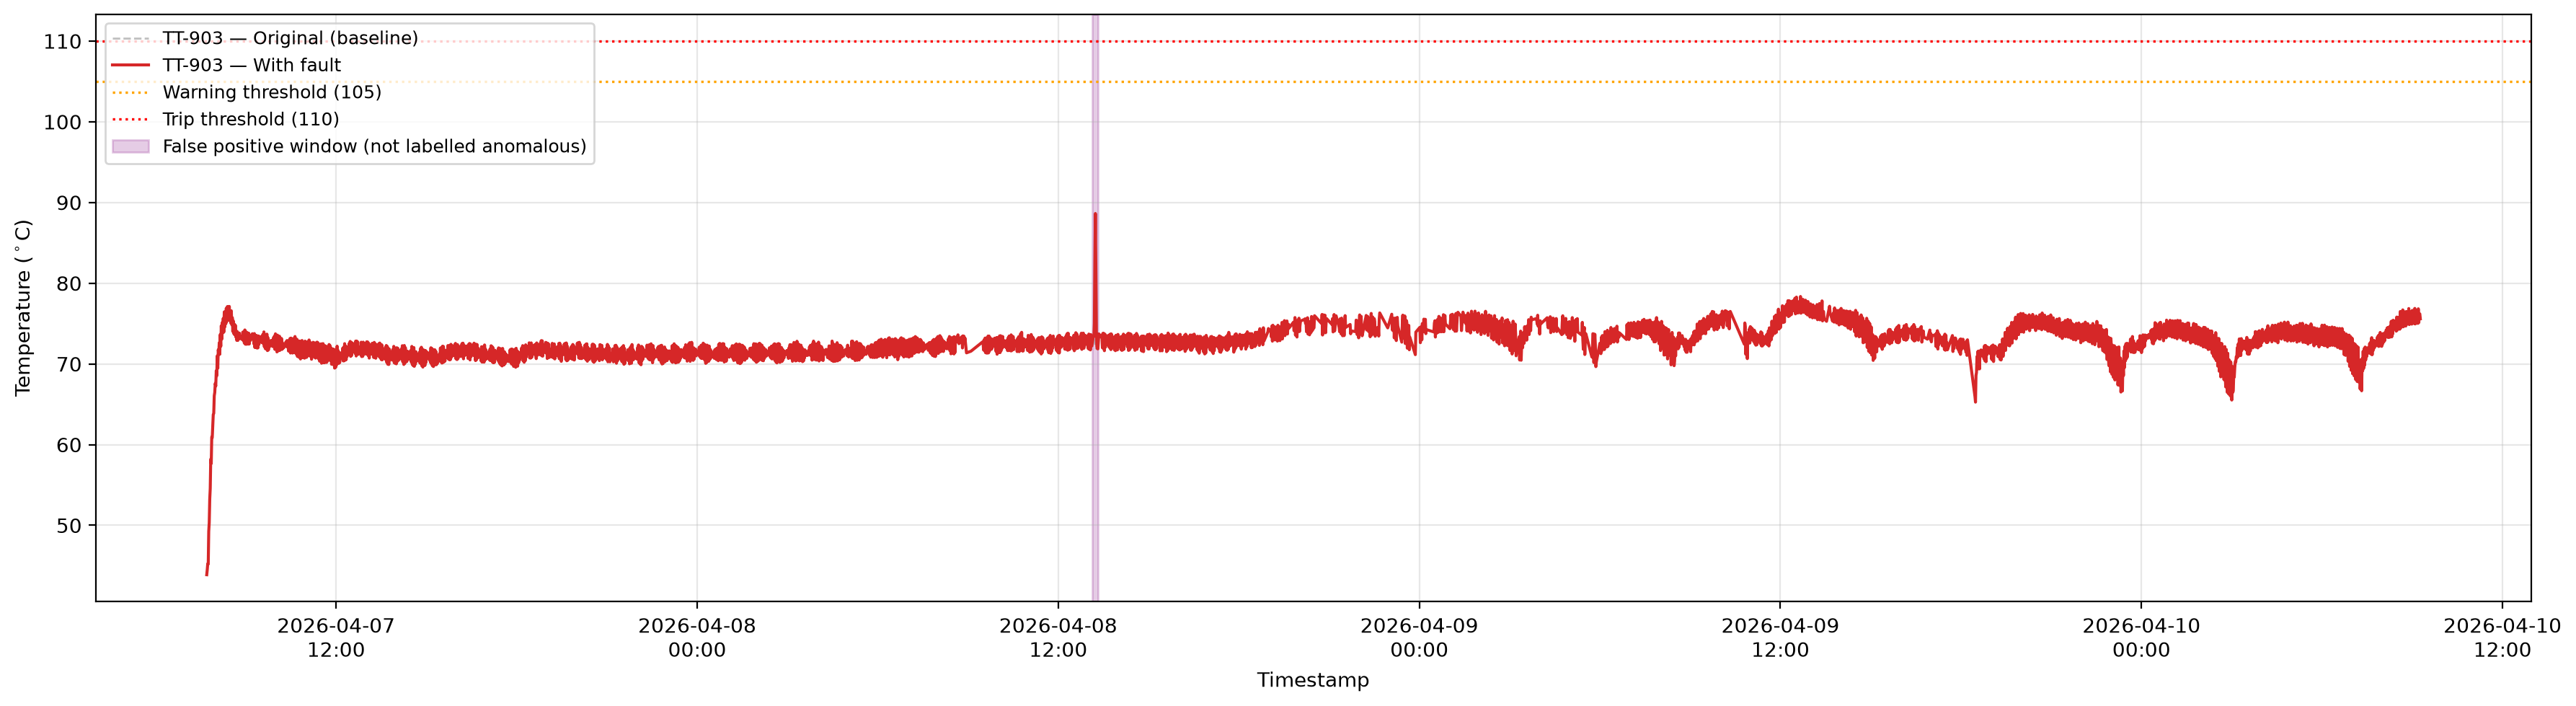
\includegraphics[width=0.95\textwidth]{imgs/fault_fp_s17.png}
    \caption{Standalone false positive scenario, Session 17: TT-903 with and without the injected spike. The spike stays below the trip threshold and is not propagated to any correlated sensor.}
    \label{fig:ap2_fp_s17}
\end{figure}